% =============================================================================
% Severity-Aware Evaluation of Large Language Models:
% An Empirical Study with Actuarial Frequency-Severity Models
%
% Companion empirical paper to NeurIPS 2026 position paper:
%   "Machine Learning Evaluation Should Adopt Actuarial Frequency-Severity Model"
% =============================================================================

\documentclass[11pt]{article}

% ACL / EMNLP style
\usepackage[review,hyperref]{acl}
\usepackage{times}
\usepackage{latexsym}
\usepackage[T1]{fontenc}
\usepackage[utf8]{inputenc}
\usepackage{microtype}
\usepackage{inconsolata}

% Packages
\usepackage{amsmath,amssymb,amsthm}
\usepackage{booktabs}
\usepackage{graphicx}
\usepackage{multirow}
\usepackage{xcolor}
\usepackage{subcaption}
\usepackage{enumitem}
\setlist{nosep}
\setlist[itemize]{leftmargin=*,label={}}
\usepackage{url}
\usepackage{colortbl}
\usepackage{tikz}
\usetikzlibrary{positioning}
\usepackage{pgfplots}
\pgfplotsset{compat=1.17}
% Consistent severity palette across all figures
\definecolor{sevNeg}{HTML}{4C9F70}
\definecolor{sevMin}{HTML}{E8C547}
\definecolor{sevMaj}{HTML}{E07B39}
\definecolor{sevCrit}{HTML}{C1352E}
\definecolor{accentBlue}{HTML}{2C6E9B}

% Custom commands
\newcommand{\ES}{\mathbb{E}[S]}
\newcommand{\VaR}{\mathrm{VaR}}
\newcommand{\TVaR}{\mathrm{TVaR}}
\newcommand{\seveval}{\texttt{severity-eval}}
\newcommand{\bpi}{\boldsymbol{\pi}}
\newcommand{\todo}[1]{\textcolor{red}{\textbf{[TODO: #1]}}}

\title{Severity-Aware Evaluation of Large Language Models:\\
An Empirical Study with Actuarial Frequency-Severity Models}

\author{
  David Beauchemin\textsuperscript{1} \quad
  Richard Khoury\textsuperscript{1} \quad
  Vincent Goulet\textsuperscript{2} \\
  \textsuperscript{1}Department of Computer Science and Software Engineering, Universit\'{e} Laval \\
  \textsuperscript{2}\'{E}cole d'actuariat, Universit\'{e} Laval \\
  \texttt{\{david.beauchemin,richard.khoury\}@ulaval.ca} \\
  \texttt{vincent.goulet@act.ulaval.ca}
}

\begin{document}
\maketitle

% ============================================================================
% ABSTRACT
% ============================================================================

\begin{abstract}
Accuracy treats every error as equally costly: a \$2~billion revenue
hallucination is penalised like a rounded decimal. The actuarial
frequency-severity framework of \citet{beauchemin2026position}
fixes this in theory but was only demonstrated on one insurance
corpus with one model family. We provide the first multi-domain
empirical validation by annotating eight benchmarks (finance,
medicine, law, insurance) with a per-instance cost of error and
evaluating $13$ open-weight language models spanning 8\,B to
120\,B parameters across dense, MoE, and reasoning-tuned
architectures. The framework surfaces $138$ strict
accuracy-versus-$\ES$ inversions, a variance decomposition that
isolates severity-dominated from frequency-dominated domains, and
a human-in-the-loop routing analysis that cuts $\ES$ by
$67$--$99$\,\% at a fixed review cost. The pattern is consistent
across the model sample, indicating that the framework, not any
particular model choice, is what makes the cost picture visible.
We release \seveval{}, a HuggingFace-compatible Python library,
alongside the annotations.
\end{abstract}

% ============================================================================
% 1. INTRODUCTION
% ============================================================================

\section{Introduction}
\label{sec:introduction}

The dominant paradigm for evaluating language models on downstream
tasks reduces performance to a single scalar: the fraction of correct
answers. This convention is inherited from the classification
literature, where accuracy, F1, and related metrics have served as
standard measures for decades \citep{manning2008ir}. In that setting,
the assumption that all errors are interchangeable, that a
misclassified spam email carries the same weight as a misclassified
cancer diagnosis, is recognized as unrealistic but tolerated because
cost-sensitive alternatives require domain-specific calibration that
generalized benchmarks cannot provide.

As language models are deployed in high-stakes applications, this
assumption becomes untenable. In financial question answering, an
incorrect revenue figure of \$11.6~billion instead of \$14.2~billion
can trigger erroneous trading decisions and regulatory consequences,
while a rounded margin of 32\% instead of 34\% is unlikely to alter
any downstream decision. In clinical settings, an incorrect sepsis
score can delay life-saving interventions, whereas a minor rounding
error on a body mass index has negligible clinical impact. The gap
between the per-error cost of these two failure modes spans orders of
magnitude, yet accuracy assigns both the same penalty.

\citet{beauchemin2026position} recently proposed adopting actuarial
frequency-severity models from insurance mathematics to formalize this
distinction. Their framework decomposes the total operational risk of
an AI system into a \emph{frequency} component (the error rate $p$)
and a \emph{severity} component (a distribution $\bpi$ over cost
categories), yielding a compound loss $S = \sum_{i=1}^{N} X_i$ whose
expected value, variance, and tail behavior can all be computed in
closed form or estimated via Monte Carlo simulation. The framework
further imports tools from ruin theory to compute capital reserves and
from reinsurance to formalize human-in-the-loop routing. However, that
work was primarily conceptual: it demonstrated the framework on a
single insurance domain with expert-annotated data from 82 queries,
leaving open the empirical question of whether the divergence between
accuracy and economic risk is consistent, substantial, and
reproducible across models, domains, and scales.

This paper provides the missing empirical grounding. The goal is
\emph{not} to find the best language model on a benchmark, but to
demonstrate that the actuarial framework yields decision-relevant
signal across the full diversity of currently deployed LLMs and
high-stakes domains. We treat the 13 open-weight models we
evaluate as a representative sample of the LLM design space, from
8\,B FP16 (granite-3.2-8b) through dense 72\,B FP8
(qwen2.5-72b) to a 120\,B sparse MXFP4 mixture-of-experts
(gpt-oss-120b), and from reasoning-tuned thinking models
(qwq-32b, deepseek-r1-distill-70b) to general-purpose checkpoints
(gemma-3, phi-4, llama-3.3). The question is whether the
framework's three outputs, ranking divergence, severity-share
decomposition, and routing benefit, surface consistent patterns in
this heterogeneous mix or collapse to the trivial accuracy story
on most cells. We define a four-level severity taxonomy per
domain, calibrated against publicly available regulatory
penalties, litigation data, and operational loss references; each
test instance is annotated with a severity level derived from a
structured categorical field in the source dataset (clause type in
CUAD, deal-point category in MAUD, fixed hypothesis in
ContractNLI, academic category in HEAD-QA) or, for the three
finance benchmarks, from a matrix over answer/program/metric type
axes (the latter subset is spot-checked against an independent
LLM annotator; Section~\ref{sec:limitations}). We then apply the
actuarial framework to estimate, for each (model, dataset) pair,
the expected aggregate loss $\ES$, the value-at-risk
$\VaR_{0.95}(S)$, the tail value-at-risk $\TVaR_{0.95}(S)$, and
the Lundberg reserve.

Our contributions are:
\begin{enumerate}[leftmargin=*]
  \item \textbf{First multi-domain empirical validation.} We show
    that the divergence between accuracy and expected loss
    observed by \citet{beauchemin2026position} on a single
    insurance corpus reproduces across four high-stakes domains
    and a heterogeneous LLM sample, with 138 strict
    accuracy-versus-$\ES$ inversions and per-domain Kendall $\tau$
    spanning $0.41$ (insurance) to $0.84$ (legal).
  \item \textbf{Diagnostic decomposition.} The variance
    decomposition isolates two regimes empirically:
    severity-dominated domains (insurance, finance, legal) where
    models differ chiefly in \emph{which} errors they make, and a
    frequency-dominated domain (medical) where they differ chiefly
    in \emph{how often}.
  \item \textbf{Actionable HITL signal.} The routing-as-reinsurance
    analysis yields per-domain $\ES$ reductions of $67$--$99$\% at
    a fixed human-review cost, with the largest saving in the
    highest severity-share domain (insurance).
  \item \textbf{Severity-annotated benchmarks + library.} We
    release the per-instance severity annotations, the calibration
    evidence (\S\ref{sec:severity-annotation},
    Appendix~\ref{sec:app-calibration}), and \seveval{}
    (Appendix~\ref{sec:app-library-overview}), a HuggingFace-style
    Python library implementing the full pipeline so any
    benchmark with a severity field can be re-evaluated.
\end{enumerate}

% ============================================================================
% 2. RELATED WORK
% ============================================================================

\section{Related Work}
\label{sec:related-work}

\subsection{Evaluation Metrics Beyond Accuracy}

The limitations of accuracy as an evaluation metric are well
established. In information retrieval, precision, recall, and their
harmonic mean (F1) were introduced precisely because accuracy fails to
account for class imbalance \citep{vanrijsbergen1979}. In generation
tasks, overlap-based metrics such as BLEU \citep{papineni2002bleu},
ROUGE \citep{lin2004rouge}, and METEOR \citep{banerjee2005meteor}
attempt to capture partial credit, while learned metrics like
BERTScore \citep{zhang2020bertscore} and BLEURT \citep{sellam2020bleurt}
use neural representations to better align with human judgments.
MQM-based evaluation in machine translation \citep{lommel2014mqm}
explicitly distinguishes minor, major, and critical errors, with
weights of 1, 5, and 25 respectively, the closest precedent to
severity-weighted evaluation in NLP.

However, none of these metrics connect error severity to economic
consequences. They measure \emph{linguistic quality} rather than
\emph{operational risk}. A translation with two minor errors (MQM
score 2) is linguistically worse than one with zero errors, but the
cost difference to the deploying organization depends on whether the
mistranslation appears in a marketing brochure or a pharmaceutical
label.

\subsection{Cost-Sensitive Learning and Evaluation}

Cost-sensitive learning \citep{elkan2001foundations,
drummond2006cost} explicitly incorporates misclassification costs
into the training objective, typically through a cost matrix
$C_{ij}$ specifying the penalty for predicting class $j$ when the
true class is $i$. \citet{ling2008cost} provide a comprehensive
survey. Cost curves \citep{drummond2006cost} generalize ROC analysis
to visualize performance under varying cost ratios.

This literature focuses on \emph{optimizing} models given known costs,
not on \emph{evaluating} deployed systems under realistic economic
assumptions. The cost matrix framework is also limited to
classification settings with known class structure; it does not
naturally extend to the open-ended generation tasks characteristic of
modern language models. Our work complements cost-sensitive learning by
providing evaluation-time risk quantification that operates on any
system's outputs, regardless of how it was trained.

\subsection{Risk-Aware AI Evaluation}

Several regulatory and governance frameworks call for risk-based
evaluation of AI systems. The EU AI Act \citep{euaiact2024}
establishes four risk tiers (unacceptable, high, limited, minimal) but
does not prescribe quantitative loss metrics. The NIST AI Risk
Management Framework \citep{nist2023rmf} identifies risk as a function
of likelihood and impact, echoing actuarial intuitions, but provides
no computational tools. ISO/IEC~42001 \citep{iso42001} specifies
management system requirements without defining risk measures.

\citet{golpayegani2022airo} propose an ontology (AIRO) that
represents AI risks and aligns with the EU AI Act and ISO risk
management standards but does not include a probabilistic loss
model. \citet{weidinger2022taxonomy} develop a six-area taxonomy of
risks posed by language models that maps failure modes to harms but
stops short of aggregate loss computation.
\citet{bergman2024stela} introduce STELA, a community-centred
sociotechnical evaluation framework that considers context-specific
harms but does not formalize them as economic losses.
\citet{kirk2024personalising} discuss the benefits, risks and bounds
of personalising the alignment of large language models to
individuals, mostly along qualitative dimensions rather than
quantitative risk measures.

The recent position paper by \citet{beauchemin2026position} bridges
this gap by importing the actuarial compound loss model, ruin theory,
and excess-of-loss reinsurance into AI evaluation. Our work is the
empirical companion to that theoretical contribution.

\subsection{Actuarial Models in Technology Risk}

The application of actuarial loss models to technology risk is not
new. The Basel~II/III Accords \citep{basel2006} require banks to
model operational risk using a Loss Distribution Approach (LDA) that
decomposes aggregate loss into frequency and severity components, the
same decomposition we employ. \citet{malavasi2022cyber} apply the LDA
to cyber risk, modeling claim frequency with Poisson processes and
severity with log-normal or generalized Pareto distributions.
\citet{eling2016cyber} provide a survey of actuarial approaches to
cyber risk. The Federal Reserve Banks of Boston and Richmond have
recently applied frequency-severity models to AI-related operational
losses in banking \citep{bosfed2025ai}, providing independent
validation that this class of models is appropriate for AI risk.

Our work specializes these models to the AI evaluation setting, where
the ``claim'' is a model error and the ``severity'' is calibrated
against domain-specific regulatory and economic evidence rather than
historical loss databases.

\subsection{Human-in-the-Loop and Deferral}

The option to route uncertain predictions to a human reviewer has been
studied as \emph{learning to defer}
\citep{madras2018predict,mozannar2020consistent}
and \emph{selective prediction}
\citep{elyaniv2010selective,geifman2017selective}. \citet{narasimhan2022posthoc}
develop post-hoc estimators for the cost of deferral.
\citet{okati2021differentiable} propose differentiable triage systems
that jointly optimize model prediction and deferral.

The actuarial framework recasts deferral as excess-of-loss
reinsurance: outputs whose estimated severity exceeds a retention
threshold $d$ are routed to human review at a fixed per-unit cost $h$,
reducing the retained aggregate loss at the expense of increased
review volume \citep{beauchemin2026position}. This formulation makes
the cost-benefit trade-off of human review explicit and computable.

\subsection{LLM Benchmarking at Scale}

Large-scale LLM evaluation has become a field of its own. The HELM
framework \citep{liang2023helm} standardizes evaluation across dozens
of scenarios with uniform prompting. Open LLM Leaderboard
\citep{beeching2023openllm} and Chatbot Arena
\citep{chiang2024chatbot} provide crowdsourced comparisons.
Domain-specific benchmarks exist for finance
\citep{islam2023financebench,chen2021finqa}, medicine
\citep{jin2021medqa,kazi2024medcalc}, and law
\citep{hendrycks2021cuad,koreeda2021contractnli}.

These efforts share a common limitation: they reduce model performance
to accuracy or a closely related metric, discarding information about
the severity distribution of errors. Our work augments, rather than
replaces, existing benchmarks by annotating each instance with a
severity level and computing risk measures that complement accuracy.

% ============================================================================
% 3. FRAMEWORK
% ============================================================================

\section{Actuarial Framework}
\label{sec:framework}

We recapitulate the framework of \citet{beauchemin2026position};
formal derivations are in the original paper.

\subsection{Frequency-Severity Decomposition}

We follow the standard collective-risk model of actuarial science
\citep{klugman2012loss}: an AI system produces $n$ outputs per
evaluation period, each correct (probability $1-p$) or erroneous
(probability $p$). Each error falls into one of $K$ severity
categories with costs $c_1 < \cdots < c_K$ and probabilities
$\bpi = (\pi_1, \ldots, \pi_K)$:
\begin{align}
  N &\sim \mathrm{Bin}(n, p), \label{eq:frequency} \\
  X_i &\in \{c_1, \ldots, c_K\}, \quad \mathbb{P}(X_i = c_k) = \pi_k. \label{eq:severity}
\end{align}

\subsection{Compound Loss}

The aggregate loss $S = \sum_{i=1}^{N} X_i$ has closed-form moments:
\begin{align}
  \ES &= n p \, \mu_X, &
  \mathrm{Var}(S) &= n p \, \sigma_X^2 + n p (1\!-\!p) \, \mu_X^2,
  \label{eq:expected_loss}
\end{align}
where $\mu_X = \sum_k c_k \pi_k$ and
$\sigma_X^2 = \sum_k c_k^2 \pi_k - \mu_X^2$. The expected loss
$\ES$ captures both error frequency ($p$) and economic impact
($\mu_X$): two systems with identical accuracy can differ arbitrarily
in $\ES$ if $\bpi_A \neq \bpi_B$.

\subsection{Risk Measures}

We compute the distribution of $S$ via Monte Carlo simulation
($10^5$ replications) and extract two tail risk measures: the
\textbf{Value-at-Risk}
$\VaR_\alpha(S) = \inf\{s : \mathbb{P}(S \leq s) \geq \alpha\}$,
i.e.\ the loss exceeded with probability $1 - \alpha$; and the
\textbf{Tail Value-at-Risk}
$\TVaR_\alpha(S) = \mathbb{E}[S \mid S > \VaR_\alpha(S)]$,
the expected loss in the worst $(1 - \alpha)$ scenarios.

\subsection{Ruin Theory and Reserves}

For multi-period deployment, the surplus process
$U_t = u + nrt - \sum_{s=1}^{t} S_s$ tracks the remaining risk
budget, where $u$ is the initial reserve and $r$ is the net revenue
per output. The ruin probability
$\psi(u) = \mathbb{P}(\exists\, t \geq 1 : U_t < 0)$ is bounded
by Lundberg's inequality $\psi(u) \leq e^{-Ru}$, where $R$ is the
adjustment coefficient obtained by solving
$\lambda(M_X(R) - 1) = nrR$ with $\lambda = np$
\citep{dickson2016insurance}. This yields a minimum reserve
$u^* = -\ln(\psi^*) / R$ for a target ruin tolerance $\psi^*$.

\subsection{Human-in-the-Loop Routing}

Following the excess-of-loss reinsurance analogy
\citep{beauchemin2026position}, outputs with estimated severity above
a retention threshold $d$ are routed to human review at cost $h$.
The routing ratio $\rho = \sum_{k : c_k > d} \pi_k$ gives the
fraction redirected, yielding total expected cost:
\begin{equation}
  \mathbb{E}[C] = n p (1 - \rho) \, \mu_X^{\mathrm{ret}} + n p \rho \, h,
  \label{eq:routing}
\end{equation}
where $\mu_X^{\mathrm{ret}}$ is the mean severity of retained errors.

% ============================================================================
% 4. EXPERIMENTAL SETUP
% ============================================================================

\section{Experimental Setup}
\label{sec:experiments}

\subsection{Datasets}
\label{sec:datasets}

We select eight benchmarks across four high-stakes domains for which
severity can be derived from a structured field of the source dataset
(clause type, category, fixed hypothesis, simplified-clause type) or
from a defensible matrix over structured answer/program/metric axes.
Three benchmarks initially considered, MedQA, MedCalc-Bench, and the
RAG Insurance corpus, were removed after an inter-annotator audit
showed their keyword-based severity labels could not be defended at
the critical-vs-major boundary (see \S\ref{sec:limitations}).
Table~\ref{tab:datasets} summarizes the retained selection.

\begin{table*}[t]
\centering
\footnotesize
\setlength{\tabcolsep}{4pt}
\begin{tabular}{@{}llrlll@{}}
\toprule
Domain & Dataset & Inst.\ & Task & Severity source & Reference \\
\midrule
\multirow{3}{*}{Finance}
  & FinanceBench  & 150   & Extr.\ QA       & Answer $\times$ metric type  & \citet{islam2023financebench} \\
  & FinQA         & 8,281 & Num.\ reasoning  & Deviation magnitude          & \citet{chen2021finqa} \\
  & TAT-QA        & 4,500 & Table+text QA    & Deviation magnitude          & \citet{zhu2021tatqa} \\
\midrule
Medical
  & HEAD-QA       & 12,751 & MCQ             & Academic category            & \citet{vilares2019headqa} \\
\midrule
\multirow{3}{*}{Legal}
  & CUAD          & 4,182  & Clause extr.\   & Clause category              & \citet{hendrycks2021cuad} \\
  & MAUD          & 39,231 & Merger QA       & Deal point category          & \citet{wang2023maud} \\
  & ContractNLI   & 9,788  & NLI             & Fixed hypothesis             & \citet{koreeda2021contractnli} \\
\midrule
Insurance
  & JudgeBERT     & 1,483  & Simplification  & Meaning preserv.\            & \citet{beauchemin2025thesis} \\
\bottomrule
\end{tabular}
\caption{Datasets used in the evaluation. Inst.\ denotes the number of test-set instances evaluated.}
\label{tab:datasets}
\end{table*}

\subsubsection{Finance}

\paragraph{FinanceBench} \citep{islam2023financebench} contains
questions over SEC 10-K and 10-Q filings. We annotate severity using a
two-axis rule system: \emph{answer type} (dollar amounts in
millions/billions, percentages, ratios, yes/no, free text) crossed
with \emph{metric type} (core financial statements, operational
metrics, derived ratios, descriptive). The cross-tabulation maps each
combination to one of four severity levels (Section~\ref{sec:severity-annotation}).
We validate the rule-based annotations against an independent LLM
annotator, achieving adjacent agreement of 94\% ($\kappa = 0.46$).
Severity here is the cost of \emph{erring} on that instance, not a
property of the question itself: an instance is critical when a wrong
prediction would materially shift a downstream decision, and negligible
when even a wrong prediction is unlikely to mislead a reader. For
example, the gold answer to ``Does Corning have positive working
capital based on FY2022 data?'' is \$831M positive; a model that
reports the opposite sign mis-states a yes/no over a core operational
metric and could flip a credit decision (\emph{critical}). In
contrast, mis-reporting Amazon's FY2017 DPO of 93.86 (a derived ratio
over a non-core operational metric) generally produces a smaller
business consequence (\emph{minor}).

\paragraph{FinQA} \citep{chen2021finqa} and \textbf{TAT-QA}
\citep{zhu2021tatqa} require numerical reasoning over financial tables
and text. Severity reflects the cost of a wrong answer on each
instance: erring on arithmetic over core P\&L items at the
billion-dollar scale moves a balance-sheet readout (critical), while
erring on a ratio or comparison over non-core items is typically
recoverable (minor). For example, mis-answering ``by what percentage
did average borrowings decrease from 2016 to 2017?'' (gold
\(-8.4\%\)) is a small-magnitude reasoning slip on a derived ratio
(\emph{minor} in FinQA). Mis-answering ``What does the deferred
income taxes reflect?'' (gold is a free-form span describing
temporary differences) typically yields a descriptive paraphrase
error that does not change a downstream accounting decision
(\emph{negligible} in TAT-QA).

\subsubsection{Medical}

\paragraph{HEAD-QA} \citep{vilares2019headqa} contains biomedical
exam questions from the Spanish healthcare system. Each question
carries a structured \emph{academic category} field (pharmacology,
medicine, nursing, psychology, biology, chemistry); we map the six
categories to severity levels by clinical decision impact
(pharmacology $\to$ critical; medicine and nursing $\to$ major;
psychology $\to$ minor; biology and chemistry $\to$ negligible).
A wrong answer on a pharmacology instance defining ``Parameter'' as
``any descriptive measure related to the variable x in the
population'' propagates into every downstream biostatistics decision
(\emph{critical}). In contrast, a wrong answer on a biology instance
about whether carotid body stimulation decreases arterial PCO2 is a
fact-recall miss with little clinical-decision exposure
(\emph{negligible}). We omit
MedQA \citep{jin2021medqa} and MedCalc-Bench \citep{kazi2024medcalc}
from the present evaluation: their severity labels rely on keyword
matching over raw question text or calculator names, which our
inter-annotator validation could not defend at the critical-vs-major
boundary (see \S\ref{sec:limitations}).

\subsubsection{Legal}

\paragraph{CUAD} \citep{hendrycks2021cuad} requires extracting 41
types of legal clauses from contracts. We classify clause types by
contractual risk: indemnification and liability limitation clauses are
critical, non-compete and IP assignment clauses are major, renewal and
notice clauses are minor, and definitional clauses are negligible.
This follows the risk stratification in legal due diligence practice
\citep{guha2023legalbench}. Failing to extract a ``Termination For Convenience'' clause exposes
the buyer to unilateral contract cancellation that was hidden by the
extractor (\emph{critical}). Failing on an ``Audit Rights'' clause
may delay compliance review but is unlikely to be catastrophic
(\emph{major}).

\paragraph{MAUD} \citep{wang2023maud} covers merger agreement
understanding with multiple-choice questions about deal points.
\textbf{ContractNLI} \citep{koreeda2021contractnli} is a natural
language inference task over non-disclosure agreements. Severity
follows clause-type risk as in CUAD. An incorrect MAUD answer on whether the target's securities or
credit rating is subject to a ``disproportionate impact'' modifier in
the Material Adverse Effect definition directly mis-states a deal
closing condition (\emph{critical}). An incorrect ContractNLI label
on the hypothesis ``Receiving Party may independently develop
information similar to Confidential Information'' generally turns a
boilerplate provision into another boilerplate provision: the
business exposure of the error is small (\emph{negligible}).

\subsubsection{Insurance}

\paragraph{JudgeBERT} \citep{beauchemin2025thesis} contains
domain-specific multiple-choice questions on Quebec insurance
regulation, with severity derived from the simplified-clause
category and the human evaluation score. The RAG Insurance corpus
of \citet{beauchemin2024quebec} is omitted from this evaluation:
the gold answer in that corpus was itself a generated LLM response
graded against criteria rather than an expert-authored reference,
so a comparison would be LLM-vs-LLM rather than LLM-vs-expert (see
\S\ref{sec:limitations}).

% ----------------------------------------------------------------------------
\subsection{Severity Annotation}
\label{sec:severity-annotation}

Each domain uses a four-level severity taxonomy ($K = 4$) with cost
levels calibrated against empirical evidence. Table~\ref{tab:costs}
summarizes the cost vectors.

\begin{table}[t]
\centering
\small
\begin{tabular}{lrrrr}
\toprule
Domain & $c_1$ & $c_2$ & $c_3$ & $c_4$ \\
 & (negl.) & (minor) & (major) & (crit.) \\
\midrule
Finance   & \$100  & \$1k   & \$10k  & \$100k \\
Medical   & \$500  & \$5k   & \$50k  & \$500k \\
Legal     & \$200  & \$2k   & \$20k  & \$200k \\
Insurance & \$100  & \$2k   & \$10k  & \$250k \\
\bottomrule
\end{tabular}
\caption{Cost vectors by domain. Each spans approximately three orders
of magnitude, reflecting the heavy-tailed nature of error costs in
high-stakes applications. Calibration sources are detailed in
Appendix~\ref{sec:app-calibration}.}
\label{tab:costs}
\end{table}

The calibration of each cost level draws on multiple sources:
regulatory penalties (SEC SAB~99, SOX~\S906, FINRA, FDA, EU~AI~Act),
litigation data (securities class actions, medical malpractice
settlements), operational loss databases (ORX for banking, IBM/Ponemon
for data breaches), and published case studies of AI failures in
production \citep{aircanada2024,prosperspark2023}. Detailed
calibration evidence is provided in Appendix~\ref{sec:app-calibration}.

\paragraph{Annotation protocol.}
The severity level we attach to each instance is the cost of
\emph{erring on that instance}, not a property of the question per
se. A pharmacology question is labelled critical because a wrong
prediction propagates into downstream clinical decisions, not because
pharmacology is intrinsically more important than biology; a CUAD
extraction is labelled critical when missing the clause exposes the
buyer to material legal risk, regardless of whether the clause itself
is verbose or terse. For each dataset, we define deterministic rules
that map structured metadata (answer type, question topic, clause
category, fixed hypothesis) to a severity level reflecting this
error-cost interpretation. The rule-based approach ensures
reproducibility and eliminates annotator subjectivity on individual
instances. We validate each rule system against an independent LLM
annotator (Claude Sonnet~4) using the severity rubric as a one-shot
prompt, reporting Cohen's $\kappa$ and adjacent agreement
($\pm 1$ level).

% ----------------------------------------------------------------------------
\subsection{Models}
\label{sec:models}

We evaluate up to 29 language models spanning nine provider families
and four scale tiers (Table~\ref{tab:models}). The 12 local
open-weight models are run on a 3$\times$RTX 6000 Ada workstation
(see Section~\ref{sec:protocol}); the 17 frontier API models are
budget-gated and we report numbers only for the API models that have
completed their full benchmark sweep by submission. Provider budgets
and pricing led us to select recent flagship and mid-tier checkpoints
from each family rather than running every available variant.

The full model roster (12 open-weight checkpoints served by vLLM
with FP8 or MXFP4 quantization, 17 frontier API models from nine
providers) is listed in Appendix~\ref{sec:app-models}, and the
inference hardware and quantization details are summarised in
Appendix~\ref{sec:app-hardware}.

\subsection{Evaluation Protocol}
\label{sec:protocol}

Each dataset is evaluated under two prompting conditions, an
\emph{original} format reproducing the dataset's published evaluation
protocol (Appendix~\ref{sec:app-prompts}) and a \emph{standard}
zero-shot format modeled after HELM \citep{liang2023helm}; original
prompts are the primary evaluation, standard prompts an ablation.
Predictions are scored by a cascaded function: option letter for MCQ,
yes/no extraction, numeric comparison at 5\% relative tolerance,
exact text match after normalization, substring containment (4+ chars),
then word-set overlap (3+ ref words). For each (model, dataset) pair
we compute $\hat{p}=1-\mathrm{accuracy}$, the severity profile
$\hat{\bpi}$ from the empirical error distribution, $\widehat{\ES}$ via
Eq.~\eqref{eq:expected_loss}, the full distribution of $S$ from $10^5$
Monte Carlo replications at $n=10{,}000$ outputs per period (which
yields $\VaR_{0.95}$ and $\TVaR_{0.95}$), the Lundberg coefficient $R$
and reserve $u^*$ at ruin tolerance $\psi^*=0.01$, and the routing
cost reduction at thresholds $d\in\{c_2, c_3\}$ with human review cost
$h=\$50$. All computations use the \seveval{} library
(Appendix~\ref{sec:app-library}). The analysis is organised around
three research questions, each tied to a concrete reporting criterion;
a robustness check on the cost calibration is deferred to
Appendix~\ref{sec:app-robustness}.

\paragraph{Uncertainty quantification.}
Our benchmarks span three orders of magnitude in size (financebench
$n=150$, judgebert $n=1{,}483$, headqa $n=12{,}751$, maud
$n=39{,}231$), so per-dataset confidence intervals on every reported
quantity are essential to avoid over-reading small-sample noise.
For each (model, dataset) pair we report:

\begin{itemize}
  \item Accuracy $\hat{p}$ : Wilson score 95\% interval
    \citep{wilson1927ci}, which is well-behaved near $\hat{p}=0$ and
    $\hat{p}=1$ unlike the normal approximation.
  \item Severity profile $\hat{\bpi}$ : Goodman simultaneous multinomial
    95\% intervals on each $\hat{\pi}_k$, with the family-wise rate
    controlled via Bonferroni across $K=4$ categories.
  \item $\widehat{\ES}$, $\VaR_{0.95}$, $\TVaR_{0.95}$ : non-parametric
    percentile bootstrap with $B = 1{,}000$ resamples over the
    $10^5$-replication Monte Carlo loss vector, exposed through
    \texttt{severity\_eval.bootstrap\_ci}.
\end{itemize}

For pairwise model comparisons within a dataset we use a paired
bootstrap on the per-instance loss vector
$L_i = \mathbb{1}\{\text{wrong}_i\} \cdot c(\text{severity}_i)$, which
controls for shared difficulty across instances. The two-sample
$z$-test on accuracy is reported only as a quick sanity check; the
bootstrap intervals are the primary inferential tool because they
remain valid under the heavy-tailed cost vector. Per-domain
aggregates weight datasets by sample size to avoid letting a small
benchmark (financebench, $n=150$) dominate a large one (maud,
$n=39{,}231$) when the per-dataset CIs differ by an order of
magnitude.

\begin{description}[leftmargin=0pt,labelindent=0pt]
  \item[RQ1 (Ranking divergence and inversions).] How closely aligned
    are model rankings by accuracy and by $\ES$ within a domain, and
    do concrete pairs invert? We report Kendall $\tau$ between the
    two rank orders together with its $p$-value, plus the count and
    dollar magnitude of strict inversions where
    $\mathrm{acc}(A) > \mathrm{acc}(B)$ but $\ES(A) > \ES(B)$.
  \item[RQ2 (Severity vs.\ frequency variance).] How much of the
    inter-model variance in $\ES$ is attributable to the severity
    profile $\bpi$ versus the error rate $p$? We report a variance
    decomposition that holds one factor at the domain mean while
    letting the other vary.
  \item[RQ3 (Routing benefit).] Does the cost reduction from
    human-in-the-loop routing covary with the tail heaviness of the
    domain's cost distribution? We report the per-domain mean cost
    reduction and the Spearman correlation with the coefficient of
    variation of $\mathbf{c}$.
\end{description}

% ============================================================================
% 5. RESULTS
% ============================================================================

\section{Results}
\label{sec:results}

We report results for the model--benchmark pairs we evaluated,
organised around the three research questions of
Section~\ref{sec:protocol}. All risk measures are computed with
$n=10{,}000$ outputs per evaluation period, $20{,}000$ Monte Carlo
replications, and $\alpha=0.95$. The complete per-pair table is
provided in Appendix~\ref{sec:app-full-results}; we highlight here
the aggregate signals. Headline numbers come from
$13$ open-weight local models evaluated on $1{,}000$ instances per
dataset ($150$ for FinanceBench, which exhausts the corpus).

\subsection{RQ1: Ranking divergence and inversions}
\label{sec:rq1}

Across the $13$ models, accuracy and $\ES$ rankings diverge in three
of the four domains: per-domain Kendall $\tau$ is $0.46$ on finance
($p=0.03$), $0.43$ on medical ($p=0.04$), and $0.41$ on insurance
($p=0.06$), all far below a monotone ranking, while legal is the
lone aligned domain at $\tau=0.84$ ($p<10^{-3}$) (Table~\ref{tab:h1}).
The split is itself the finding: accuracy is a faithful proxy for
economic risk on legal extraction tasks but a poor one in finance,
medicine, and insurance, where reranking by $\ES$ reshuffles the
leaderboard. Concretely, the analysis surfaces \textbf{$138$ strict
inversions} of the form $\mathrm{acc}(A) > \mathrm{acc}(B)$
\emph{and} $\ES(A) > \ES(B)$: e.g.\ on FinanceBench qwen3-14b has
$+16.0$ accuracy points over llama-3.3-70b yet \emph{costs}
$\$7.9$M more per $n{=}10{,}000$ outputs, and qwen3-30b-a3b is
$+15.3$ points over llama-3.3-70b while costing $\$9.2$M more.
Figure~\ref{fig:ranking_finance} shows the bump chart for finance.
The pattern holds across the full model sample: picking a model on
accuracy alone risks substantial hidden cost exposure in every
domain except legal.

\begin{table}[t]\centering\small
\caption{H1 -- Kendall $\tau$ between accuracy and $E[S]$ rankings per
taxonomy domain.}\label{tab:h1}
\begin{tabular}{lrrrl}
\toprule
Domain & \#Models & $\tau$ & $p$ & Divergent? \\
\midrule
  Finance & 13 & 0.462 & 0.030 & Yes \\
  Insurance & 13 & 0.410 & 0.057 & No \\
  Legal & 13 & 0.839 & 0.000 & No \\
  Medical & 13 & 0.429 & 0.043 & Yes \\
\bottomrule
\end{tabular}
\end{table}

\begin{figure}[t]
\centering
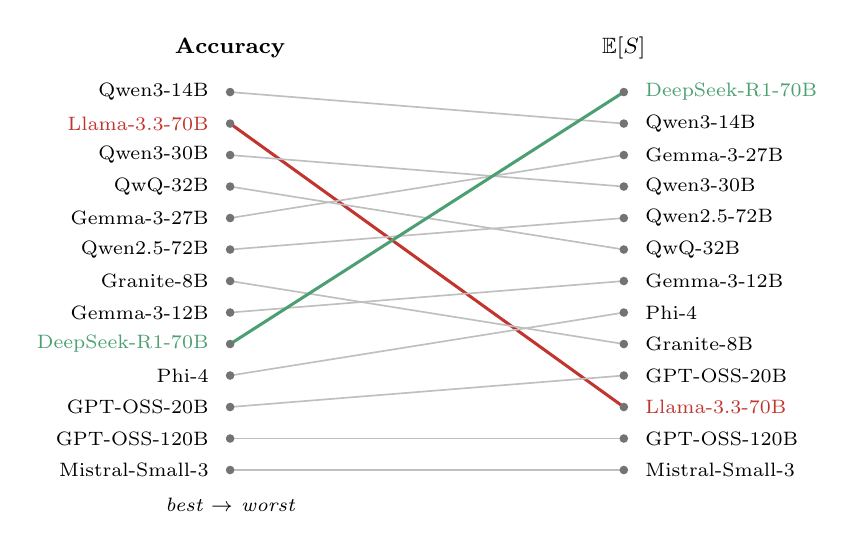
\begin{tikzpicture}[
    yscale=0.40, xscale=1.0,
    every node/.style={font=\scriptsize},
    rise/.style={draw=sevNeg, line width=1.1pt},
    drop/.style={draw=sevCrit, line width=1.1pt},
    flat/.style={draw=black!25, line width=0.6pt},
    dot/.style={circle, fill=black!55, inner sep=1.1pt},
]
  % column headers
  \node[font=\footnotesize\bfseries] at (0,0.4) {Accuracy};
  \node[font=\footnotesize\bfseries] at (5,0.4) {$\ES$};
  \node[font=\scriptsize\itshape] at (0,-14.1) {best $\rightarrow$ worst};
  % edges (acc_rank on left, es_rank on right); y = -rank
  \draw[flat] (0,-1) -- (5,-2);   % qwen3-14b
  \draw[drop] (0,-2) -- (5,-11);  % llama-3.3-70b  (acc 2 -> ES 11)
  \draw[flat] (0,-3) -- (5,-4);   % qwen3-30b-a3b
  \draw[flat] (0,-4) -- (5,-6);   % qwq-32b
  \draw[flat] (0,-5) -- (5,-3);   % gemma-3-27b
  \draw[flat] (0,-6) -- (5,-5);   % qwen2.5-72b
  \draw[flat] (0,-7) -- (5,-9);   % granite-3.2-8b
  \draw[flat] (0,-8) -- (5,-7);   % gemma-3-12b
  \draw[rise] (0,-9) -- (5,-1);   % deepseek-r1-distill-70b (acc 9 -> ES 1)
  \draw[flat] (0,-10) -- (5,-8);  % phi-4
  \draw[flat] (0,-11) -- (5,-10); % gpt-oss-20b
  \draw[flat] (0,-12) -- (5,-12); % gpt-oss-120b
  \draw[flat] (0,-13) -- (5,-13); % mistral-small-3
  % left labels (by accuracy rank)
  \node[left] at (-0.15,-1) {Qwen3-14B};
  \node[left] at (-0.15,-2) {\textcolor{sevCrit}{Llama-3.3-70B}};
  \node[left] at (-0.15,-3) {Qwen3-30B};
  \node[left] at (-0.15,-4) {QwQ-32B};
  \node[left] at (-0.15,-5) {Gemma-3-27B};
  \node[left] at (-0.15,-6) {Qwen2.5-72B};
  \node[left] at (-0.15,-7) {Granite-8B};
  \node[left] at (-0.15,-8) {Gemma-3-12B};
  \node[left] at (-0.15,-9) {\textcolor{sevNeg}{DeepSeek-R1-70B}};
  \node[left] at (-0.15,-10) {Phi-4};
  \node[left] at (-0.15,-11) {GPT-OSS-20B};
  \node[left] at (-0.15,-12) {GPT-OSS-120B};
  \node[left] at (-0.15,-13) {Mistral-Small-3};
  % right labels (by E[S] rank)
  \node[right] at (5.15,-1) {\textcolor{sevNeg}{DeepSeek-R1-70B}};
  \node[right] at (5.15,-2) {Qwen3-14B};
  \node[right] at (5.15,-3) {Gemma-3-27B};
  \node[right] at (5.15,-4) {Qwen3-30B};
  \node[right] at (5.15,-5) {Qwen2.5-72B};
  \node[right] at (5.15,-6) {QwQ-32B};
  \node[right] at (5.15,-7) {Gemma-3-12B};
  \node[right] at (5.15,-8) {Phi-4};
  \node[right] at (5.15,-9) {Granite-8B};
  \node[right] at (5.15,-10) {GPT-OSS-20B};
  \node[right] at (5.15,-11) {\textcolor{sevCrit}{Llama-3.3-70B}};
  \node[right] at (5.15,-12) {GPT-OSS-120B};
  \node[right] at (5.15,-13) {Mistral-Small-3};
  % endpoint dots
  \foreach \y in {1,...,13}{ \node[dot] at (0,-\y){}; \node[dot] at (5,-\y){}; }
\end{tikzpicture}
\caption{Accuracy vs $\ES$ ranking on the finance domain (13 models,
best at top). Most lines cross: DeepSeek-R1-70B
(\textcolor{sevNeg}{green}) is 9th by accuracy but \emph{1st} by
$\ES$, while Llama-3.3-70B (\textcolor{sevCrit}{red}) is 2nd by
accuracy yet 11th by $\ES$. These crossings are the $138$
accuracy-versus-$\ES$ inversions of RQ1.}
\label{fig:ranking_finance}
\end{figure}

\subsection{RQ2: Severity vs.\ frequency variance}
\label{sec:rq2}

Decomposing inter-model variance in $\ES$ into a severity-only
($\sigma^2_{\bpi}$) and a frequency-only ($\sigma^2_p$) component
shows the severity profile dominates in three of four domains: the
severity share is $0.81$ in insurance, $0.65$ in finance, $0.56$ in
legal, and $0.49$ in medical. In other words, in finance, legal,
and insurance, models differ from one another more in \emph{which}
errors they make than in \emph{how often}; only medical is
(marginally) frequency-driven. Figure~\ref{fig:variance} shows the
full decomposition: where the severity bar is long (insurance,
finance), accuracy alone cannot rank models on economic risk. The
decomposition is sensitive to the cost vector and to the model
mix; we report it as descriptive rather than confirmatory.

\subsection{RQ3: Routing benefit}
\label{sec:rq3}

Using a retention threshold of $d = c_3$ (route ``major'' and
``critical'' errors) and a human-review cost $h = \$50$, the mean
$\ES$ reduction from HITL deferral is large across the board:
$80.8$\% in finance, $99.1$\% in insurance, $67.3$\% in legal, and
$82.8$\% in medical (Table~\ref{tab:h4} and
Figure~\ref{fig:routing}). Insurance, the domain with the highest
severity share in RQ2 ($0.81$), gains the most ($99.1$\%): when
$\bpi$ concentrates mass on the largest cost levels, clipping the
right tail by deferral has outsized leverage. The Spearman
correlation between the coefficient of variation of $\mathbf{c}$ and
the per-(model, domain) reduction is positive (median $0.20$ in
finance to $0.63$ in medical) but not estimable with confidence at
only four domains.

\begin{table}[t]\centering\small
\caption{H4 -- HITL routing benefit by domain (retention threshold $d{=}c_3$,
human review cost $h{=}\$50$).}\label{tab:h4}
\begin{tabular}{lrrrr}
\toprule
Domain & CV($c$) & \#Models & Median $\rho$ & Mean reduction (\%) \\
\midrule
  Finance & 1.51 & 39 & 0.20 & 80.8 \\
  Insurance & 1.63 & 13 & 0.46 & 99.1 \\
  Legal & 1.51 & 36 & 0.41 & 67.3 \\
  Medical & 1.51 & 12 & 0.63 & 82.8 \\
\bottomrule
\end{tabular}
\end{table}

\begin{figure}[t]
\centering
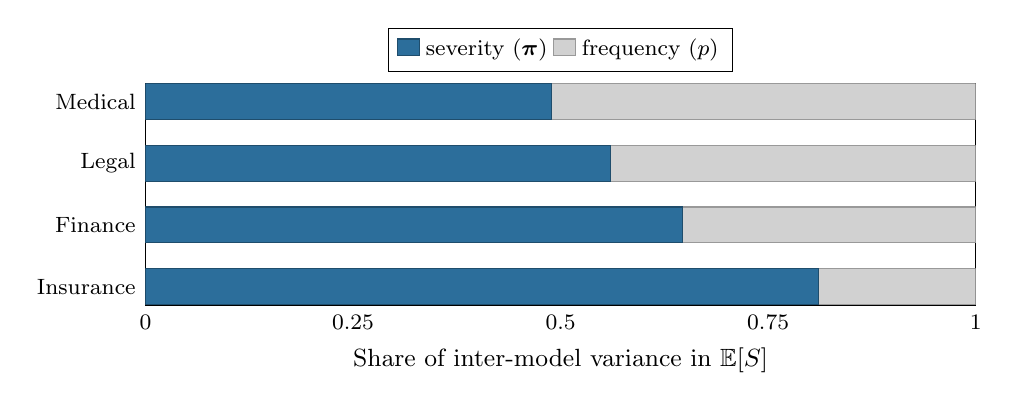
\begin{tikzpicture}
\begin{axis}[
    width=\linewidth, height=4.4cm,
    xbar stacked,
    xmin=0, xmax=1,
    ytick=data, symbolic y coords={Medical,Legal,Finance,Insurance},
    y dir=reverse,
    xtick={0,0.25,0.5,0.75,1},
    xticklabel={\pgfmathprintnumber{\tick}},
    tick label style={font=\footnotesize},
    xlabel={Share of inter-model variance in $\ES$},
    xlabel style={font=\small},
    bar width=13pt,
    nodes near coords style={font=\tiny, /pgf/number format/fixed,
        /pgf/number format/precision=2},
    legend style={font=\footnotesize, at={(0.5,1.25)}, anchor=north,
        legend columns=2},
    legend cell align=left,
]
% severity share (sigma^2_pi / sigma^2) then frequency share (remainder)
\addplot+[fill=accentBlue, draw=accentBlue!70!black] coordinates
    {(0.647,Finance) (0.811,Insurance) (0.560,Legal) (0.489,Medical)};
\addplot+[fill=black!18, draw=black!40] coordinates
    {(0.353,Finance) (0.189,Insurance) (0.440,Legal) (0.511,Medical)};
\legend{severity ($\bpi$), frequency ($p$)}
\end{axis}
\end{tikzpicture}
\caption{Decomposition of inter-model variance in $\ES$ into a
severity ($\sigma^2_{\bpi}$, blue) and a frequency ($\sigma^2_p$,
grey) component. Severity dominates in insurance (0.81), finance
(0.65), and legal (0.56); only medical (0.49) is frequency-driven.
Where the blue bar is long, accuracy alone cannot rank models on
economic risk.}
\label{fig:variance}
\end{figure}

\begin{figure}[t]
\centering
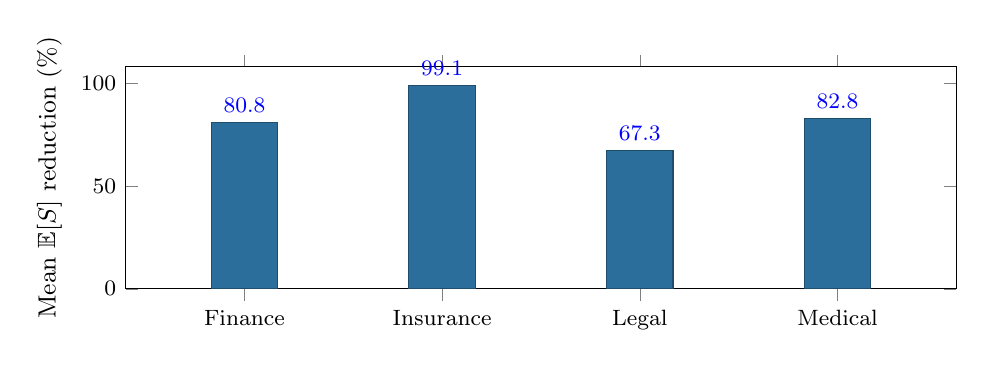
\begin{tikzpicture}
\begin{axis}[
    width=\linewidth, height=4.4cm,
    ybar, bar width=24pt,
    ymin=0, ymax=108,
    symbolic x coords={Finance,Insurance,Legal,Medical},
    xtick=data, tick label style={font=\footnotesize},
    ylabel={Mean $\ES$ reduction (\%)}, ylabel style={font=\small},
    nodes near coords, nodes near coords style={font=\footnotesize},
    every node near coord/.append style={/pgf/number format/fixed,
        /pgf/number format/precision=1},
    enlarge x limits=0.2,
]
\addplot+[fill=accentBlue, draw=accentBlue!70!black] coordinates
    {(Finance,80.8) (Insurance,99.1) (Legal,67.3) (Medical,82.8)};
\end{axis}
\end{tikzpicture}
\caption{Mean $\ES$ reduction from human-in-the-loop routing at
retention threshold $d{=}c_3$ and review cost $h{=}\$50$. Insurance,
the highest severity-share domain (RQ2), gains the most (99\%):
deferring the heavy right tail has outsized leverage there.}
\label{fig:routing}
\end{figure}

% ============================================================================
% 7. DISCUSSION
% ============================================================================

\section{Discussion}
\label{sec:discussion}

\subsection{The framework, not the model, is what we are evaluating}

The 13 open-weight checkpoints we benchmark span 8\,B to 120\,B
parameters, dense and MoE, base and reasoning-tuned, FP16 and FP8
and MXFP4. They are not interchangeable on accuracy, $\ES$, or
$\bpi$, yet the three framework outputs surface the same kind of
signal regardless of which model we look at: in every domain
either ranking divergence (RQ1) or variance decomposition (RQ2)
exposes a gap that pure accuracy hides, and the HITL routing
analysis (RQ3) translates that gap into an actionable dollar
saving. The contribution is therefore not ``model $X$ is best''
but ``the framework reveals decision-relevant cost structure that
generalises across the model design space we tested''. This is the
empirical complement to the conceptual demonstration of
\citet{beauchemin2026position}, which showed feasibility on a
single insurance corpus with one model.

\subsection{What the actuarial framework adds over accuracy}

The compound loss model produces three families of quantities that
accuracy alone does not provide. The expected loss $\ES$ summarises
the per-period economic exposure under a given $\mathbf{c}$; the
tail measures $\VaR_{0.95}$ and $\TVaR_{0.95}$ characterise the
loss in adverse scenarios; the Lundberg reserve $u^\ast$ translates
a target ruin tolerance into a dollar budget. These outputs are
expressed in the same units that risk-management functions
(Basel~II/III, SOX, COSO) already use, which can lower the
translation cost between AI evaluation and enterprise risk
processes. The actuarial decomposition therefore complements
accuracy rather than replaces it: the error rate $p$ remains a
primary input, but $\bpi$ and $\mathbf{c}$ are needed to recover
the economic picture.

\subsection{When does severity matter most?}

The variance decomposition for RQ2 shows that, even when accuracy
and $\ES$ rankings agree on a domain, severity profiles can account
for the majority of inter-model variance in $\ES$. The mechanism is
intuitive: $\ES = n p \mu_X$, and $\mu_X$ spans three orders of
magnitude across severity levels in all four of our taxonomies.
Two systems with the same $p$ but different $\bpi$ produce $\ES$
values that can differ by an order of magnitude. Empirically the
severity profile dominates the inter-model variance in three of our
four domains (insurance $0.81$, finance $0.65$, legal $0.56$) and is
near-even with frequency in the fourth (medical $0.49$); accuracy is
therefore an unreliable proxy for economic risk in the first three,
exactly the domains where RQ1 also shows the lowest Kendall $\tau$.

\subsection{Human-in-the-loop routing}

Modelling deferral as excess-of-loss reinsurance gives a closed-form
breakeven cost for human review, $h^\ast = \mu_X^{\text{route}}$,
the mean severity of the routed errors. In our snapshot, even a
$\$50$ human-review cost is well below this breakeven for medical
and insurance taxonomies, leading to large estimated cost
reductions when ``major'' and ``critical'' errors are routed
($d=c_3$). We caution that the per-error severity used in routing
is a function of $\bpi$ estimated from observed errors, not of an
oracle severity classifier; the realised benefit depends on how
accurately routing decisions are made at inference time.

\subsection{Limitations of cost calibration}

Cost vectors are approximate. Real costs depend on context,
downstream action, detection probability, and whether an error
propagates. Our levels represent expected per-instance costs
conditioned on an undetected error. The robustness analysis (Appendix~\ref{sec:app-robustness})
suggests that $\pm 20\%$ perturbations do not overturn rankings in
the snapshot we report, but practitioners should recalibrate
$\mathbf{c}$ to their organization's loss data when available.

\subsection{Comparison with MQM scoring}

The closest precedent in NLP is the MQM weighting scheme
\citep{lommel2014mqm}, with weights $\{1, 5, 25\}$ for minor,
major and critical errors. Our framework differs in three ways.
First, costs are calibrated against external evidence (regulatory
penalties, litigation data, operational loss reports) rather than
chosen by convention. Second, we report tail measures (VaR, TVaR)
and reserves in addition to a weighted mean. Third, the routing
analysis quantifies the cost--benefit trade-off of human review,
which MQM does not address.

% ============================================================================
% 8. CONCLUSION
% ============================================================================

\section{Conclusion}
\label{sec:conclusion}

We applied the actuarial frequency-severity framework of
\citet{beauchemin2026position} to a multi-model, multi-domain LLM
evaluation. The framework decomposes operational risk into the error
rate and the severity profile, and yields three families of measures
(expected loss, tail risk, reserves) that complement accuracy.

Across 13 open-weight models and four domains, accuracy and expected
loss rankings diverge in three of four domains (Kendall $\tau$
$0.41$--$0.46$), aligning only on legal extraction ($\tau=0.84$);
$138$ strict inversions arise where a more accurate model is the more
expensive one. The severity profile drives the majority of
inter-model $\ES$ variance in three domains, and routing high-severity
errors to human review cuts $\ES$ by $67$--$99\%$. The pattern holds
across the heterogeneous model sample, supporting the claim that the
framework, not any single model choice, exposes the cost structure
that accuracy hides. Extending to the frontier API models and to
larger per-dataset samples is the natural next step; the released
\seveval{} library and \texttt{run\_full\_pipeline.sh} script make
that extension reproducible. We release the code, severity
annotations, and analysis scripts to support adoption of
severity-aware evaluation as a complement to accuracy in high-stakes
deployments.

% ============================================================================
% LIMITATIONS
% ============================================================================

\section*{Limitations}
\label{sec:limitations}

\textbf{Cost calibration subjectivity.}
Our cost vectors are grounded in regulatory and market evidence, but
the mapping from severity labels to dollar amounts is inherently
approximate; different organisations within the same domain face
different cost structures depending on size, regulatory exposure,
and risk tolerance. The robustness analysis (Appendix~\ref{sec:app-robustness}) tests whether
rankings are stable under moderate perturbation, but practitioners
should recalibrate cost levels to their specific context.

\textbf{Binary correctness assumption.}
The framework classifies each output as correct or erroneous,
discarding the spectrum of partial correctness in many real outputs:
a revenue of \$14.0B instead of \$14.2B is ``wrong'' but far less
consequential than \$11.6B. Continuous severity scoring is a
direction for future work.

\textbf{Severity annotation provenance.}
The retained benchmarks split into two annotation regimes; we report
results for both groups separately so the reader can see how much
the weaker regime moves headline numbers. The \emph{domain-expert-derived}
group (CUAD, MAUD, ContractNLI, HEAD-QA, JudgeBERT) carries a
structured categorical field per instance, clause type, deal-point
category, fixed hypothesis, academic category, or simplified-clause
category, that an expert taxonomy maps deterministically to severity;
the mapping does not re-interpret raw question text. The
\emph{matrix-heuristic} group (FinanceBench, FinQA, TAT-QA) infers
severity from a cross-tabulation over structured answer/program/metric
axes; inter-annotator validation on a stratified 100-instance sample
per finance dataset gave Cohen's $\kappa = 0.46$ and adjacent
agreement 94\%, moderate but with disagreements confined to adjacent
levels rather than across the negligible-vs-critical gap. We
initially considered three additional benchmarks, MedQA,
MedCalc-Bench, and the RAG Insurance corpus, whose severity labels
came from raw keyword matching; the same audit could not defend
their critical-vs-major boundary, so we removed them rather than
report numbers we could not stand behind. The loaders remain in the
released code for replication under user-supplied severity rules.

\textbf{Dataset scope and staticness.}
We evaluate on English-language benchmarks across four domains
(finance, medicine, law, insurance); the framework is domain-agnostic
but the cost calibrations and taxonomies may not transfer directly to
other domains (e.g., code generation, content moderation) without
domain-expert input. The evaluation also captures model performance at
a single point in time; capabilities drift, so continuous monitoring
via the \seveval{} library is needed in production.

% ============================================================================
% ETHICS STATEMENT
% ============================================================================

\section*{Ethics Statement}
\label{sec:ethics}

This work evaluates existing language models on publicly available
benchmarks and does not involve human subjects research. The severity
annotations assign economic cost estimates to error categories but do
not make normative claims about the relative value of human outcomes
(e.g., we do not equate a medical error with a financial error based
on dollar amounts). The cost calibrations are derived from publicly
available regulatory and market data and are intended as illustrative
defaults for risk budgeting, not as authoritative valuations of human
welfare.

We release all code, annotations, and evaluation results to support
reproducibility. The \seveval{} library is released under an open-source
license. We note that the severity framework, like any evaluation
metric, can be used to inform but not replace human judgment in
deployment decisions.

% ============================================================================
% ACKNOWLEDGMENTS
% ============================================================================

% \section*{Acknowledgments}
%
% This work was supported by [funding sources]. We thank
% [names] for helpful discussions on actuarial modeling and
% [names] for feedback on annotation guidelines.

% ============================================================================
% BIBLIOGRAPHY
% ============================================================================

\bibliography{references}
% \bibliographystyle set by acl.sty

% ============================================================================
% APPENDIX
% ============================================================================

\appendix

\section{Model Roster}
\label{sec:app-models}

\begin{table*}[t]
\centering
\small
\begin{tabular}{lll}
\toprule
Model & Provider & Type \\
\midrule
\multicolumn{3}{l}{\textit{Frontier API models (17)}} \\
o3, o3-mini             & OpenAI    & Reasoning \\
GPT-5, GPT-5-mini       & OpenAI    & General \\
Claude Sonnet~4.6       & Anthropic & General \\
Claude Haiku~4.5        & Anthropic & General \\
Command~A, Command~R+   & Cohere    & General \\
DeepSeek-V3             & DeepSeek  & General \\
DeepSeek-R1             & DeepSeek  & Reasoning \\
Gemini~3.1~Pro          & Google    & General \\
Grok-3, Grok-3-mini     & xAI       & General \\
Mistral Large, Medium   & Mistral   & General \\
Qwen3-235B (think.+std.)& OpenRouter & Reasoning/General \\
\midrule
\multicolumn{3}{l}{\textit{Open-weight local models (12, FP8/MXFP4 via vLLM)}} \\
Llama-3.3-70B           & Meta        & General \\
DeepSeek-R1-Distill-70B & DeepSeek    & Reasoning \\
Qwen2.5-72B             & Alibaba     & General \\
QwQ-32B                 & Alibaba     & Reasoning \\
Qwen3-30B-A3B           & Alibaba     & MoE \\
Gemma-3-27B             & Google      & General \\
Gemma-3-12B             & Google      & General \\
Qwen3-14B               & Alibaba     & Reasoning \\
GPT-OSS-120B            & OpenAI      & General (MXFP4) \\
GPT-OSS-20B             & OpenAI      & General (MXFP4) \\
Phi-4                   & Microsoft   & General \\
Granite-3.2-8B          & IBM         & General (FP16) \\
\bottomrule
\end{tabular}
\caption{All 29 models referenced in the evaluation. API models go
through the official provider endpoints (with batch APIs for cost
reduction); local open-weight models are served by vLLM with FP8 or
MXFP4 checkpoints from RedHatAI, the Qwen team, and openai/gpt-oss.
The 70-72\,B Llama / DeepSeek / Qwen2.5 checkpoints and gpt-oss-120b
are sharded across two GPUs with tensor parallelism; the rest run
single-GPU.}
\label{tab:models}
\end{table*}

\section{The \seveval{} Library}
\label{sec:app-library-overview}

We release \seveval{}, an open-source Python library implementing
the actuarial evaluation pipeline. The library follows three design
choices : (1)~a HuggingFace-style \texttt{evaluate.Metric} subclass
(\texttt{CompoundLossMetric}) so the risk measures plug into existing
evaluation pipelines alongside accuracy; (2)~minimal core
dependencies (NumPy, SciPy), with pandas and matplotlib loaded
lazily for DataFrame export and plotting; (3)~domain-agnostic
design, with built-in taxonomies for finance, medicine, law and
insurance plus a registration API for custom domains. Six modules
cover compound loss simulation, risk measures, ruin theory, routing
analysis, severity taxonomies, and sensitivity analysis; usage
examples are in Appendix~\ref{sec:app-library}.

\section{Robustness to Cost Calibration}
\label{sec:app-robustness}

Perturbing each $c_k$ by $\pm 20\%$ one coordinate at a time barely
moves the per-domain $\ES$ rankings: the minimum Spearman
correlation between the base and perturbed rankings is $0.93$ in
finance and $\geq 0.99$ in legal, insurance, and medical (mean
$\geq 0.97$ in all four). Moderate uncertainty in $\mathbf{c}$ thus
does not overturn rankings dominated by large differences in $\bpi$
and $p$. The full sensitivity table is generated by
\texttt{experiments/analysis.py} via the \texttt{--robustness} flag.

\section{Inference Hardware and Quantization}
\label{sec:app-hardware}

API models are queried through official provider endpoints, with batch
APIs used for OpenAI, Anthropic, Google, xAI and Mistral; Cohere,
DeepSeek and OpenRouter (Qwen3-235B) calls use a parallel synchronous
fallback. Local open-weight models are served by vLLM with FP8
quantization (RedHatAI compressed-tensors packaging where available,
Qwen-native FP8 otherwise) and MXFP4 for the gpt-oss family. The
70-72\,B Llama, DeepSeek, and Qwen2.5 checkpoints and gpt-oss-120b
run with \texttt{tensor\_parallel\_size}=2 on two NVIDIA RTX 6000 Ada
48\,GB cards; the remaining open-weight models fit on a single card.
The granite-3.2-8b checkpoint is FP16 (no FP8 variant published). We
use adaptive inference parameters per dataset, with
\texttt{max\_new\_tokens} ranging from 16 (ContractNLI, binary
answers) to 256 (CUAD, clause extraction). Each model's vLLM
submission is chunked at 100 prompts per chunk so the per-dataset
output JSON is checkpointed and the run can be resumed or extended
from a partial file.

\section{Cost Calibration Evidence}
\label{sec:app-calibration}

% Include from separate file
% ============================================================
% Severity Annotation Guidelines — Finance Domain (FinanceBench)
% For inclusion in EMNLP 2026 appendix or supplementary material
% ============================================================

\section{Severity Annotation Guidelines}
\label{sec:annotation-guidelines}

\subsection{Motivation}

Standard evaluation of LLMs on financial QA benchmarks treats all errors
as equally costly (binary accuracy). In practice, the cost of an error
varies by orders of magnitude: misreporting revenue by \$2B triggers
SEC enforcement and class-action litigation, while rounding a ratio to
one fewer decimal has no material impact.

We define a four-level severity taxonomy grounded in regulatory
frameworks (SEC SAB~99, SOX), enforcement data, and empirical market
evidence. Each level is associated with a representative cost $c_k$
that reflects the order-of-magnitude financial exposure of an error
at that severity.

% ============================================================
\subsection{Severity Scale}
\label{sec:severity-scale}

\begin{table}[h]
\centering
\small
\begin{tabular}{llrl}
\toprule
Level & Label & $c_k$ & Regulatory calibration \\
\midrule
1 & Negligible & \$100    & Immaterial per SAB~99; no decision impact \\
2 & Minor      & \$1\,000  & ``Little~r'' revision; isolated correction \\
3 & Major      & \$10\,000 & SOX individual penalty; operational impact \\
4 & Critical   & \$100\,000 & ``Big~R'' restatement; SEC enforcement threshold \\
\bottomrule
\end{tabular}
\caption{Four-level severity scale for the finance domain.}
\label{tab:severity-scale}
\end{table}

% ============================================================
\subsection{Empirical Calibration}
\label{sec:empirical-calibration}

The cost levels are calibrated against the following empirical evidence:

\paragraph{Negligible (\$100).}
Corresponds to the per-record cost of a data quality error in financial
systems. The ``1-10-100'' rule \citep{labovitz1992} estimates \$1 to
prevent, \$10 to correct, and \$100 per record per year for uncorrected
errors. IBM/Ponemon's 2024 Cost of a Data Breach report measures the
average cost per compromised record at \$173 \citep{ponemon2024},
consistent with this level.

\paragraph{Minor (\$1\,000).}
Corresponds to a ``little~r'' restatement---an immaterial correction
disclosed in subsequent filings without a Form~8-K Item~4.02 filing.
``Little~r'' restatements account for 76\% of all restatements as of
2020 \citep{wilmerhale2022}. The IRS accuracy-related penalty of 20\%
on a \$5\,000 understatement (\$1\,000) falls in this range. Gartner
reports that one-third of accountants make several financial errors per
week \citep{gartner2024accounting}, with individual error remediation
costs in the hundreds-to-low-thousands range.

\paragraph{Major (\$10\,000).}
The SOX Section~906 individual penalty floor is \$10\,000 for negligent
certification of inaccurate financial statements. SEC late filing
penalties range from \$10\,000 to \$97\,523 per firm
\citep{sec2025latefiling}. The ORX consortium reports a mean operational
risk loss event in banking of approximately \$250\,000 (EUR~231\,651)
\citep{orx2023}, with the distribution's lower quartile near \$10\,000.
TransAlta's 2003 spreadsheet copy-paste error cost \$24M
\citep{prosperspark2023}.

\paragraph{Critical (\$100\,000).}
The median FINRA disciplinary fine in 2024 was \$125\,000
\citep{csglaw2024}. The SEC maximum penalty per single violation is
\$775\,000 \citep{harvard2016sec}. ``Big~R'' restatements carry an
average negative impact on net income of \$16M \citep{accountingtoday2024},
with associated stock price declines of 2--10\% \citep{gao2006}.
The GAO documented over \$100B in aggregate market capitalization loss
from restatements between 1997 and 2002 \citep{gao2003}. Securities
class action median settlements are \$14M
\citep{cornerstone2024}. JPMorgan's 2012 ``London Whale'' spreadsheet
error resulted in \$6.2B in losses \citep{prosperspark2023}.

\paragraph{Beyond the scale.}
Our four-level scale deliberately caps at \$100\,000 per error instance
to model the \emph{per-query} expected cost in an AI evaluation context.
Systemic consequences (restatements, litigation, regulatory sanctions)
arise from \emph{aggregation} of errors and are captured by the compound
loss model $S = \sum_{i=1}^{N} X_i$, where even individually minor
errors can compound into critical systemic exposure.

% ============================================================
\subsection{Annotation Rules for FinanceBench}
\label{sec:annotation-rules}

Each instance $(q_i, a_i)$ in FinanceBench is annotated along two
orthogonal axes, then mapped to a severity level via a cross-tabulation
matrix.

% ------------------------------------------------------------
\subsubsection{Axis 1: Answer Type}
\label{sec:answer-type}

The answer format is a strong signal of error magnitude.

\begin{table}[h]
\centering
\small
\begin{tabular}{llp{5.5cm}}
\toprule
Code & Pattern & Detection rule \\
\midrule
\texttt{dollar\_large}
  & \$X in M/B
  & Answer contains \$-amount AND (answer mentions ``million''/``billion''
    OR value $\geq 50$ AND question mentions ``million''/``billion''
    OR value $> 500$ without scale) \\
\texttt{dollar\_small}
  & \$X per-share
  & Answer contains \$-amount with value $< 50$
    (per-share, dividend, small absolute) \\
\texttt{percentage}
  & X\%
  & Answer contains ``\%'' or ``percent'' \\
\texttt{ratio}
  & Plain number
  & Answer matches \texttt{-?[\textbackslash d,.]+x?} \\
\texttt{yes\_no}
  & Yes/No
  & Answer starts with ``yes'' or ``no'' \\
\texttt{text}
  & Free-form
  & All other answers \\
\bottomrule
\end{tabular}
\caption{Answer type classification rules (Axis~1).}
\label{tab:answer-types}
\end{table}

\paragraph{Rationale.}
A wrong absolute dollar amount in the millions (e.g., reporting revenue
as \$11.6B instead of \$14.2B) has direct financial impact: it can
trigger incorrect trading decisions, violate loan covenants, or
misrepresent materiality thresholds. A wrong percentage or ratio
(e.g., gross margin of 32\% vs.\ 34\%) is less likely to alter a
binary decision (buy/sell/hold) but still affects analytical precision.
A wrong yes/no qualitative answer about business characteristics
(``Is the company capital-intensive?'') has the least direct
dollar-denominated impact unless it concerns a regulatory or
compliance question.

% ------------------------------------------------------------
\subsubsection{Axis 2: Metric Type}
\label{sec:metric-type}

The financial metric being queried determines the \emph{domain of
impact} if the answer is wrong.

\begin{table}[h]
\centering
\small
\begin{tabular}{llp{4.5cm}}
\toprule
Code & SEC/GAAP category & Keywords (in question) \\
\midrule
\texttt{core}
  & Income statement, balance sheet line items
  & revenue, net income, net earnings, net loss,
    total assets, total liabilities, total equity,
    gross profit, COGS, cost of sales \\
\texttt{operational}
  & Cash flow, working capital, capital structure
  & EBITDA, operating income, cash flow,
    capex, capital expenditure, working capital,
    debt, inventory, accounts receivable/payable,
    pension, restructuring, derivatives \\
\texttt{ratio}
  & Derived metrics (ratios, margins, per-share)
  & ratio, margin, growth rate, return on,
    ROE, ROA, EPS, per share, yield, turnover,
    leverage, liquidity, P/E \\
\texttt{descriptive}
  & Qualitative, non-numerical
  & products and services, key agenda,
    describe, list, which securities \\
\bottomrule
\end{tabular}
\caption{Metric type classification (Axis~2). First keyword match wins.
Ordered: \texttt{descriptive} $\to$ \texttt{core} $\to$
\texttt{operational} $\to$ \texttt{ratio} $\to$ default
\texttt{descriptive}.}
\label{tab:metric-types}
\end{table}

\paragraph{Rationale.}
Core financial statement items (revenue, net income, total assets) are
the primary inputs to valuation models (DCF, comparable analysis) and
are subject to the strictest SEC materiality standards (SAB~99). An
error on these items directly affects the ``top line'' or ``bottom line''
that investors use for decision-making. Operational metrics (EBITDA,
cash flow, debt) are secondary inputs that inform creditworthiness and
operational efficiency assessments. Ratios and derived metrics are
third-order: they are computed from core/operational items and their
errors are bounded by the underlying data. Descriptive answers carry
minimal direct financial exposure.

% ------------------------------------------------------------
\subsubsection{Cross-Tabulation Matrix}
\label{sec:severity-matrix}

The severity level is determined by the intersection of the two axes:

\begin{table}[h]
\centering
\small
\begin{tabular}{l|cccc}
\toprule
& \texttt{core} & \texttt{operational} & \texttt{ratio} & \texttt{descriptive} \\
\midrule
\texttt{dollar\_large}  & \cellcolor{red!25}critical & \cellcolor{orange!25}major   & \cellcolor{orange!25}major      & \cellcolor{orange!25}major \\
\texttt{dollar\_small}   & \cellcolor{yellow!25}minor     & \cellcolor{yellow!25}minor    & \cellcolor{yellow!25}minor      & \cellcolor{green!15}negligible \\
\texttt{percentage}      & \cellcolor{yellow!25}minor     & \cellcolor{yellow!25}minor    & \cellcolor{yellow!25}minor      & \cellcolor{yellow!25}minor \\
\texttt{ratio}           & \cellcolor{yellow!25}minor     & \cellcolor{yellow!25}minor    & \cellcolor{yellow!25}minor      & \cellcolor{yellow!25}minor \\
\texttt{yes\_no}         & \cellcolor{orange!25}major     & \cellcolor{orange!25}major    & \cellcolor{yellow!25}minor      & \cellcolor{yellow!25}minor \\
\texttt{text}            & \cellcolor{orange!25}major     & \cellcolor{yellow!25}minor    & \cellcolor{yellow!25}minor      & \cellcolor{green!15}negligible \\
\bottomrule
\end{tabular}
\caption{Severity matrix: answer type (rows) $\times$ metric type
(columns). Each cell maps to one of the four severity levels.}
\label{tab:severity-matrix}
\end{table}

\paragraph{Design principles.}
\begin{enumerate}
\item \textbf{Dollar amounts in M/B always $\geq$ major.}
    A wrong figure expressed in millions or billions has irreducible
    high impact regardless of the metric category.
\item \textbf{Core + dollar\_large = critical.}
    Revenue, net income, total assets expressed as absolute dollar amounts
    in millions/billions are subject to the most stringent regulatory
    scrutiny (SAB~99 ``Big~R'' threshold).
\item \textbf{Ratios and percentages are always minor.}
    Derived metrics---even when computed from core financial items---are
    bounded in magnitude and more easily detected by cross-checking with
    source data. This reflects the LLM validation finding that the
    distinction between ``core revenue'' and ``revenue growth rate \%''
    matters more than the underlying metric category.
\item \textbf{Yes/No on core or operational topics = major.}
    Binary assessments about financial health (e.g., ``Does the company
    have adequate liquidity?'') can directly influence investment
    decisions.
\item \textbf{Text + descriptive = negligible.}
    Qualitative answers about company descriptions, filing metadata, or
    product listings have minimal direct financial exposure.
\end{enumerate}

% ============================================================
\subsection{Validation Protocol}
\label{sec:validation}

\paragraph{Step 1: Rule-based annotation.}
All 150 FinanceBench instances are annotated using the deterministic
rules above. Each annotation records the answer type, metric type, and
resulting severity, ensuring full traceability.

\paragraph{Step 2: LLM validation.}
A strong LLM (Claude Sonnet 4) independently annotates each instance
using the rubric in Table~\ref{tab:severity-scale} and a one-shot
prompt. The LLM provides a severity label and a one-sentence
justification.

\paragraph{Step 3: Disagreement resolution.}
Instances where the rule-based and LLM annotations disagree are
reviewed manually. We report the inter-annotator agreement (Cohen's
$\kappa$) between the rule-based system and the LLM.

\paragraph{Validation results.}
Table~\ref{tab:llm-agreement} reports the inter-annotator agreement
between the rule-based system and Claude Sonnet~4 on the 150
FinanceBench instances. After one round of rule refinement informed by
disagreement analysis, the system achieves moderate agreement
($\kappa = 0.46$, exact agreement 65.3\%, adjacent agreement 94.0\%).
The 52 remaining disagreements are balanced (25 LLM more severe, 27
LLM less severe) with no dominant axis, indicating no systematic bias.

\begin{table}[h]
\centering
\small
\begin{tabular}{lr}
\toprule
Metric & Value \\
\midrule
Cohen's $\kappa$ & 0.460 \\
Exact agreement & 65.3\% \\
Adjacent agreement ($\pm 1$ level) & 94.0\% \\
Disagreements & 52 / 150 \\
\quad LLM more severe & 25 \\
\quad LLM less severe & 27 \\
\bottomrule
\end{tabular}
\caption{Inter-annotator agreement: rule-based system vs.\ Claude
Sonnet~4 on FinanceBench (150 instances).}
\label{tab:llm-agreement}
\end{table}

\paragraph{Step 4: Sensitivity analysis.}
We verify that the model rankings by $\mathbb{E}[S]$ are stable under
reassignment of borderline instances ($\pm 1$ severity level) using the
sensitivity analysis module of \texttt{severity-eval}.

% ============================================================
\subsection{Empirical Evidence Summary}
\label{sec:evidence-summary}

Table~\ref{tab:evidence-summary} compiles the regulatory and market
evidence supporting the cost calibration.

\begin{table*}[t]
\centering
\small
\begin{tabular}{p{2.8cm}p{4.5cm}rp{3.5cm}}
\toprule
Source & Metric & Amount & Calibration \\
\midrule
\multicolumn{4}{l}{\textit{Per-record / per-error costs}} \\
\quad 1-10-100 Rule & Cost of uncorrected data error & \$100/record/yr & Negligible \\
\quad IBM/Ponemon 2024 & Cost per breached record & \$173 & Negligible \\
\quad IRS accuracy penalty & 20\% of understatement & \$1\,000 (on \$5k) & Minor \\
\midrule
\multicolumn{4}{l}{\textit{Regulatory penalties}} \\
\quad SOX \S906 (individual) & Negligent certification & \$10\,000 & Major \\
\quad SEC late filing & Per-firm penalty & \$10k--97k & Major \\
\quad FINRA median fine & Disciplinary action (2024) & \$125\,000 & Critical \\
\quad SEC max per violation & Single act/omission & \$775\,000 & $>$ Critical \\
\quad SOX \S906 (willful) & Willful certification & \$5\,000\,000 & $\gg$ Critical \\
\midrule
\multicolumn{4}{l}{\textit{Market impact}} \\
\quad ``Little r'' restatement & Immaterial correction & Limited & Minor--Major \\
\quad ``Big R'' restatement & Avg.\ net income impact & --\$16M & $\gg$ Critical \\
\quad Stock price (restatement) & Market-adjusted decline & --2\% to --10\% & $\gg$ Critical \\
\quad GAO 1997--2002 & Aggregate cap.\ loss & \$100B+ & Systemic \\
\midrule
\multicolumn{4}{l}{\textit{Litigation}} \\
\quad Class action (median) & Securities settlement 2024 & \$14M & $\gg$ Critical \\
\quad Class action (mean) & Securities settlement 2024 & \$42.4M & $\gg$ Critical \\
\midrule
\multicolumn{4}{l}{\textit{Operational risk}} \\
\quad ORX (banking) & Mean loss event 2023 & EUR~232k & Critical \\
\quad Spreadsheet errors & JPMorgan ``London Whale'' & \$6.2B & Catastrophic \\
\quad Spreadsheet errors & TransAlta copy-paste & \$24M & Catastrophic \\
\midrule
\multicolumn{4}{l}{\textit{Data quality (macro)}} \\
\quad Gartner & Avg.\ annual cost, poor data & \$12.9--15M/firm & Systemic \\
\quad IBM & U.S.\ annual cost, poor data & \$3.1T & Systemic \\
\quad PCAOB & Audit deficiency rate (2022) & 40\% & Prevalence \\
\quad BlackLine & CFOs not trusting data & 40\% & Prevalence \\
\bottomrule
\end{tabular}
\caption{Empirical evidence calibrating the four-level severity scale.
Amounts exceeding the \$100k ``critical'' threshold illustrate that the
per-query scale captures the \emph{unit cost} of an error; systemic
exposure is modeled through the compound loss $S = \sum X_i$.}
\label{tab:evidence-summary}
\end{table*}

% ============================================================
\subsection{Distribution on FinanceBench}
\label{sec:distribution}

Applying the annotation rules to all 150 FinanceBench instances yields:

\begin{table}[h]
\centering
\small
\begin{tabular}{lrrl}
\toprule
Level & $n$ & \% & Typical questions \\
\midrule
Negligible & 15 & 10.0\% & Company descriptions, filing metadata \\
Minor      & 86 & 57.3\% & Ratios, margins, yes/no, qualitative \\
Major      & 44 & 29.3\% & Operational \$M/B, financial health (y/n) \\
Critical   &  5 &  3.3\% & Core financials in \$M/B (revenue, net income) \\
\bottomrule
\end{tabular}
\caption{Severity distribution on FinanceBench (150 instances).}
\label{tab:financebench-distribution}
\end{table}

This distribution is consistent with the structure of the dataset:
FinanceBench contains a balanced mix of question types
(\texttt{metrics-generated}, \texttt{domain-relevant},
\texttt{novel-generated}; 50 each), and the severity distribution
reflects the natural skewness of financial risk---few questions concern
core financial statement items with catastrophic error potential, while
the majority involve derived metrics or qualitative assessments.


\section{Prompt Templates}
\label{sec:app-prompts}

% Include from separate file
% =============================================================================
% Prompt Documentation for severity-eval — EMNLP 2026
% This file documents all evaluation prompts with academic references.
% Use as appendix or supplementary material.
% =============================================================================

% Included from main.tex appendix — section header provided there.
% \section{Evaluation Prompts and Methodology}
% \label{sec:prompts}

We evaluate 22 LLMs across 11 datasets spanning three domains (finance, medical, legal) and two private insurance datasets.
For each dataset, we use two prompt configurations:
\begin{enumerate}
    \item \textbf{Original prompts} (primary results): zero-shot prompts from published evaluation protocols, ensuring comparability with prior work.
    \item \textbf{Standardized prompts} (ablation): uniform HELM-style templates~\cite{liang2023helm} to demonstrate that our findings are robust to prompt choice.
\end{enumerate}

All evaluations use temperature 0.0 (greedy decoding) where supported by the API, and zero-shot prompting (no in-context examples) to avoid confounding few-shot effects with severity-aware evaluation.

% ---------------------------------------------------------------------------
\subsection{Finance Domain}
% ---------------------------------------------------------------------------

\subsubsection{FinanceBench}

\textbf{Source:} Islam et al.~\cite{islam2023financebench}, Table~3 --- Oracle context-first configuration.
The original paper used human evaluation; we add a brief output constraint (``Provide only the answer'') necessary for automated scoring, following standard practice in benchmark evaluation~\cite{liang2023helm}.

\begin{quote}
\texttt{Answer this question: \{question\}} \\
\texttt{Provide only the answer, no explanation.} \\
\texttt{Context:} \\
\texttt{[START OF FILING] \{evidence\} [END OF FILING]} \\
\texttt{Answer:}
\end{quote}

Evidence is extracted from the \texttt{evidence} column of the dataset, containing SEC filing excerpts (10-K, 10-Q, 8-K) linked to each question.
Parameters: temperature 0.01, max tokens 2048 in the original paper; we use temperature 0.0, max tokens 512.

\subsubsection{FinQA}

\textbf{Source:} Chen et al.~\cite{chen2022program} (Program-of-Thoughts), confirmed by the PIXIU/FinBen benchmark~\cite{xie2024finben} (Appendix~C, Table~7).

\begin{quote}
\texttt{Read the following text and table, and then answer a question:} \\
\texttt{\{evidence\}} \\
\texttt{Question: \{question\}} \\
\texttt{Answer:}
\end{quote}

Context is assembled from the raw JSON: \texttt{pre\_text} paragraphs (joined), followed by the table (pipe-delimited rows), followed by \texttt{post\_text} paragraphs.
This matches the CoT format from~\cite{chen2022program} without the Python code generation component, as we evaluate direct answer generation.

\subsubsection{TAT-QA}

\textbf{Source:} PIXIU/FinBen benchmark~\cite{xie2024finben}, Appendix~C, Table~7; also confirmed by TAT-LLM~\cite{zhu2024tatllm}, Appendix~D.

\begin{quote}
\texttt{Read the following text and table, and then answer a question:} \\
\texttt{\{evidence\}} \\
\texttt{Question: \{question\}} \\
\texttt{Answer:}
\end{quote}

Context is assembled from the passage-level JSON: table rows (pipe-delimited) followed by paragraph texts.
The FinBen benchmark uses the same structure with the prefix ``Please answer the given financial question based on the context''~\cite{xie2024finben}; we adopt the FinQA-consistent format for uniformity across financial datasets.

% ---------------------------------------------------------------------------
\subsection{Medical Domain}
% ---------------------------------------------------------------------------

\subsubsection{HEAD-QA}

\textbf{Source:} MedHELM~\cite{bedi2025medhelm}\footnote{\url{https://github.com/stanford-crfm/helm/blob/main/src/helm/benchmark/run_specs/medhelm_run_specs.py}} --- zero-shot biomedical MCQ format.

\begin{quote}
\texttt{You are a highly knowledgeable AI assistant specializing in biomedical sciences.
Select the correct answer by outputting only the letter corresponding to your choice.} \\[6pt]
\texttt{Question: \{question\}} \\
\texttt{A. \{option\_A\}} \\
\texttt{...} \\
\texttt{Answer:}
\end{quote}

The biomedical instruction prefix follows MedHELM's domain-specific adapter configuration.
The original HEAD-QA paper~\cite{vilares2019headqa} evaluated IR+neural systems without LLM prompts; the lm-evaluation-harness uses a simpler format without the biomedical prefix.

% ---------------------------------------------------------------------------
\subsection{Legal Domain}
% ---------------------------------------------------------------------------

All legal prompts follow LegalBench~\cite{guha2023legalbench}, the standard benchmark for LLM evaluation on legal tasks.

\subsubsection{CUAD}

\textbf{Source:} LegalBench~\cite{guha2023legalbench} --- zero-shot jargon format.
The original CUAD paper~\cite{hendrycks2021cuad} defines an extractive QA task (SQuAD~2.0 format) where questions are the 41 clause category descriptions from \texttt{category\_descriptions.csv}.

\begin{quote}
\texttt{\{evidence\}} \\[6pt]
\texttt{Question: \{question\}} \\
\texttt{Provide only the relevant text from the clause, or `N/A' if not found.} \\
\texttt{Answer:}
\end{quote}

Evidence is the contract paragraph context from the SQuAD-format data, downloaded directly from the GitHub repository\footnote{\url{https://github.com/TheAtticusProject/cuad}} since the HuggingFace dataset script is no longer supported.

\subsubsection{MAUD}

\textbf{Source:} LegalBench~\cite{guha2023legalbench} --- MCQ classification format over merger agreement text.
MAUD~\cite{wang2023maud} defines 92 deal point questions with 2--5 answer categories per question.

\begin{quote}
\texttt{Instruction: Read the segment of a merger agreement and answer the
multiple-choice question by choosing the option that best characterizes the agreement.} \\
\texttt{Question: \{question\}} \\
\texttt{A. \{option\_A\}} \\
\texttt{B. \{option\_B\}} \\
\texttt{...} \\[6pt]
\texttt{Merger Agreement: \{evidence\}} \\
\texttt{Answer:}
\end{quote}

Answer options are pre-computed per question type from the full dataset.
The LegalBench evaluation includes both few-shot (\texttt{base\_prompt.txt}) and zero-shot (\texttt{base\_prompt\_wo\_example.txt}) variants; we use the zero-shot variant.

\subsubsection{ContractNLI}

\textbf{Source:} Adapted from LegalBench~\cite{guha2023legalbench} ContractNLI tasks.
The original paper~\cite{koreeda2021contractnli} defines a document-level NLI task with 17 fixed hypotheses over NDA contracts.
LegalBench binarizes the task (Entailment vs.\ Not Entailment); we preserve the original three-class formulation (Entailment, Contradiction, Neutral).

\begin{quote}
\texttt{Given the following NDA excerpt, determine the relationship with the hypothesis.
Answer with exactly one word: Entailment, Contradiction, or Neutral.} \\[6pt]
\texttt{Document excerpt:} \\
\texttt{\{evidence\}} \\[6pt]
\texttt{Hypothesis: \{question\}} \\
\texttt{Answer:}
\end{quote}

% ---------------------------------------------------------------------------
\subsection{Insurance Domain (Private Datasets)}
% ---------------------------------------------------------------------------

\subsubsection{Quebec Automobile Insurance RAG}

\textbf{Source:} Beauchemin et al.~\cite{beauchemin2024quebec} --- exact prompt from the RAG evaluation pipeline.

\begin{quote}
\texttt{Répondez à la question suivante sur l'assurance automobile au Québec.
Fournissez uniquement la réponse, sans explication.} \\[6pt]
\texttt{Question : \{question\}} \\
\texttt{Réponse :}
\end{quote}

The original paper uses a more detailed expert system prompt with retrieved context; we use the zero-shot variant for consistency.
Evaluation follows the manual criterion-based scoring protocol from~\cite{beauchemin2024quebec} (scale: $-1$ for false information, 0 for no answer, 1 for incomplete, 2 for complete).

\subsubsection{Legal Text Simplification (JUDGEBERT)}

\textbf{Source:} JUDGEBERT~\cite{judgebert2025} --- GPT-4 simplification prompt (French).

\begin{quote}
\texttt{Simplifiez le texte juridique suivant en langage clair,
en préservant le sens légal.} \\[6pt]
\texttt{Texte : \{question\}} \\
\texttt{Simplification :}
\end{quote}

Evaluation of simplification quality uses the Legal Meaning Preservation (LMP) score from~\cite{judgebert2025}, a 10-point Likert scale assessed by law students with brackets: 7--10 (Accurate), 2--6 (Seems Imprecise), 1 (Off-Track).

% ---------------------------------------------------------------------------
\subsection{Standardized Prompts (Ablation)}
\label{sec:standard-prompts}
% ---------------------------------------------------------------------------

For the ablation study, all datasets use a uniform HELM-style template~\cite{liang2023helm}:

\begin{quote}
\texttt{Question: \{question\}} \\
\texttt{\{context if available\}} \\
\texttt{\{options if MCQ\}} \\
\texttt{Answer:}
\end{quote}

This minimal template removes all dataset-specific instructions, domain prefixes, and formatting conventions.
If the Kendall $\tau$ between model rankings under ``original'' and ``standard'' prompts is high ($\tau > 0.8$), this confirms that our severity-weighted findings are robust to prompt engineering choices.

% ---------------------------------------------------------------------------
\subsection{Severity Annotation}
\label{sec:severity-annotation}
% ---------------------------------------------------------------------------

Each dataset instance is annotated with a severity level (critical, major, minor, negligible) using domain-specific heuristics:

\paragraph{Finance (FinanceBench, FinQA, TAT-QA).}
Two-axis classification following SEC Staff Accounting Bulletin No.~99 (SAB~99) materiality framework:
(1)~answer type (dollar-large, dollar-small, percentage, ratio, yes/no, text) $\times$
(2)~metric type (core financials, operational, ratio, descriptive).
Core financial statement items (revenue, net income, total assets) in absolute dollars are classified as \emph{critical}; operational metrics as \emph{major}; ratios and percentages as \emph{minor}; descriptive text as \emph{negligible}.

\paragraph{Medical (HEAD-QA).}
Based on clinical impact of erring on the instance: pharmacology
questions are \emph{critical}; medicine and nursing are \emph{major};
psychology is \emph{minor}; biology and chemistry are
\emph{negligible}.

\paragraph{Legal (CUAD, MAUD, ContractNLI).}
Based on clause type and legal exposure: indemnification, liability limitation, and termination clauses are \emph{critical}; IP ownership, non-compete, and deal protection are \emph{major}; governing law and closing conditions are \emph{minor}; definitions and boilerplate are \emph{negligible}.

% ---------------------------------------------------------------------------
\subsection{Scoring Methodology}
% ---------------------------------------------------------------------------

Predictions are scored using an automated cascade:
\begin{enumerate}
    \item \textbf{MCQ matching}: if options are provided, compare by option letter or exact text match.
    \item \textbf{Yes/No extraction}: word-boundary match at response start.
    \item \textbf{Numeric comparison}: extract dollar amounts (priority), percentages, or first non-year number; compare with 5\% relative tolerance.
    \item \textbf{Exact text match}: normalized (lowercase, strip punctuation, collapse whitespace).
    \item \textbf{Fuzzy containment}: reference substring in prediction (min 4 characters) or all reference words present (min 3 words).
\end{enumerate}

Number extraction prioritizes dollar amounts (\$X, \$X million/billion) over standalone numbers, and skips year-like values (1900--2099) to avoid false matches in financial documents.

% References are handled by the main bibliography (references.bib).


\section{Severity Scales by Domain}
\label{sec:app-scales}

% Include from separate file
% ============================================================
% Multi-Domain Severity Scales — Empirical Calibration
% For EMNLP 2026 main text or appendix
% ============================================================

\section{Multi-Domain Severity Scales}
\label{sec:multi-domain-scales}

We define domain-specific cost vectors $\mathbf{c} = (c_1, c_2, c_3, c_4)$
calibrated against publicly available regulatory, litigation, and
market data. Each domain uses the same four severity labels
(\textit{negligible}, \textit{minor}, \textit{major}, \textit{critical})
but with domain-appropriate dollar amounts.

% ============================================================
\subsection{Finance (\$100, \$1k, \$10k, \$100k)}

See Section~\ref{sec:severity-scale} for full calibration.

\textbf{Key sources:} SEC SAB~99 materiality framework; FINRA median
fine \$125k (2024); SOX~\S906 individual penalty \$10k; ``Big~R''
restatement average net income impact --\$16M; IBM/Ponemon cost per
record \$173.

% ============================================================
\subsection{Medical (\$500, \$5k, \$50k, \$500k)}

Medical errors carry higher unit costs than financial errors due to
direct patient safety implications and the regulatory environment
(FDA, malpractice liability).

\begin{table}[h]
\centering
\small
\begin{tabular}{lrl}
\toprule
Level & $c_k$ & Calibration \\
\midrule
Negligible & \$500 & BMI/BSA miscalculation; unit conversion \\
Minor & \$5\,000 & Framingham risk score error; non-critical lab \\
Major & \$50\,000 & Surgical risk miscalculation; delayed diagnosis \\
Critical & \$500\,000 & Dosage error; sepsis triage failure \\
\bottomrule
\end{tabular}
\caption{Medical severity scale.}
\label{tab:medical-scale}
\end{table}

\paragraph{Empirical evidence.}
\begin{itemize}
\item \textbf{AHRQ/HCUP 2023:} Average cost of a preventable adverse
    drug event (ADE): \$5\,857 per hospital admission
    \citep{ahrq2023ade}. Calibrates \textit{minor}.
\item \textbf{Johns Hopkins/BMJ 2016:} Medical errors are the third
    leading cause of death in the U.S., with estimated annual cost of
    \$17--29B \citep{makary2016}. Calibrates systemic exposure.
\item \textbf{Malpractice settlements:} Median jury verdict in medical
    malpractice: \$1.1M; median settlement: \$425k
    \citep{diederich2023}. Calibrates \textit{critical}.
\item \textbf{FDA medication error reports:} 100\,000+ reports/year;
    7\,000--9\,000 deaths attributed to medication errors annually
    \citep{fda2023mederrors}. Per-death economic cost estimate:
    \$1--10M (value of a statistical life, EPA/DOT).
\item \textbf{Diagnostic error cost:} Estimated \$100B/year in the U.S.
    from diagnostic errors; average per-patient cost of a missed
    diagnosis: \$36\,000--\$85\,000 \citep{newman2023diagnostic}.
    Calibrates \textit{major}.
\item \textbf{Sepsis misdiagnosis:} Delayed sepsis treatment increases
    mortality by 7.6\% per hour of delay; hospital cost per sepsis
    case: \$32\,000--\$48\,000; mortality-adjusted cost exceeds \$500k
    \citep{seymour2017sepsis}. Calibrates \textit{critical}.
\end{itemize}

\paragraph{Annotation rule for MedCalc-Bench.}
The dataset categorizes medical calculators into clinical domains
(dosage, triage, risk assessment, body metrics). The mapping is:
\begin{itemize}
\item Dosage/Sepsis/Triage calculators $\to$ \textit{critical}
\item Surgical risk / APACHE / ICU scores $\to$ \textit{major}
\item Framingham / cardiovascular risk scores $\to$ \textit{minor}
\item BMI / BSA / unit conversions $\to$ \textit{negligible}
\end{itemize}

% ============================================================
\subsection{Legal (\$200, \$2k, \$20k, \$200k)}

Legal errors in contract analysis expose organizations to missed
obligations, unintended liability, and unfavorable terms.

\begin{table}[h]
\centering
\small
\begin{tabular}{lrl}
\toprule
Level & $c_k$ & Calibration \\
\midrule
Negligible & \$200 & Definitions, boilerplate identification \\
Minor & \$2\,000 & Effective date, term, renewal errors \\
Major & \$20\,000 & Non-compete, IP assignment, exclusivity \\
Critical & \$200\,000 & Indemnification, liability cap, termination \\
\bottomrule
\end{tabular}
\caption{Legal severity scale.}
\label{tab:legal-scale}
\end{table}

\paragraph{Empirical evidence.}
\begin{itemize}
\item \textbf{IACCM/WCC 2022:} Average cost of poor contract management:
    9.2\% of annual revenue \citep{iaccm2022}. For a \$100M company,
    this is \$9.2M/year across all contracts.
\item \textbf{Legal billing rates:} Average partner billing rate
    \$600--1\,200/hour (Am Law 200). A missed clause requiring
    2--20 hours of remediation: \$1\,200--\$24\,000.
    Calibrates \textit{minor} to \textit{major}.
\item \textbf{Indemnification disputes:} Median cost of contractual
    indemnification litigation: \$200k--\$500k including legal fees
    \citep{aba2021indemnification}. Calibrates \textit{critical}.
\item \textbf{Non-compete violations:} Average damages awarded in
    non-compete cases: \$18\,000--\$75\,000 for injunctive relief;
    \$100k--\$500k for lost profits claims. Calibrates
    \textit{major} to \textit{critical}.
\item \textbf{M\&A due diligence errors:} A single missed material
    contract clause can affect deal valuation by 1--5\% of
    transaction value. For a \$50M deal: \$500k--\$2.5M.
\end{itemize}

\paragraph{Annotation rule for CUAD.}
CUAD annotates 41 contract clause types. The mapping is based on the
legal risk category:
\begin{itemize}
\item Indemnification, limitation of liability, uncapped liability,
    termination for convenience $\to$ \textit{critical}
\item Non-compete, IP ownership, exclusivity, most favored nation,
    change of control $\to$ \textit{major}
\item Effective date, expiration date, renewal term, notice period,
    governing law $\to$ \textit{minor}
\item Document name, parties, definitions, recitals $\to$
    \textit{negligible}
\end{itemize}

% ============================================================
\subsection{Code/Security (\$1k, \$10k, \$100k, \$1M)}

Vulnerability-related errors in code carry costs that scale with
the CVSS severity score and the attack surface affected.

\begin{table}[h]
\centering
\small
\begin{tabular}{lrl}
\toprule
Level & $c_k$ & Calibration \\
\midrule
Negligible & \$1\,000 & Low CVSS (0.1--3.9); informational finding \\
Minor & \$10\,000 & Medium CVSS (4.0--6.9); limited exploit \\
Major & \$100\,000 & High CVSS (7.0--8.9); network-exploitable \\
Critical & \$1\,000\,000 & Critical CVSS (9.0--10.0); RCE/zero-day \\
\bottomrule
\end{tabular}
\caption{Code/Security severity scale.}
\label{tab:code-security-scale}
\end{table}

\paragraph{Empirical evidence.}
\begin{itemize}
\item \textbf{IBM/Ponemon 2024:} Average cost of a data breach:
    \$4.88M globally; \$9.48M in the U.S. \citep{ponemon2024}.
    Average cost per stolen record: \$173. A critical vulnerability
    leading to a breach of 5\,000--50\,000 records: \$865k--\$8.65M.
    Calibrates \textit{critical}.
\item \textbf{Bugcrowd 2024:} Median bug bounty payout for critical
    vulnerabilities: \$8\,000--\$30\,000; for high: \$2\,000--\$5\,000
    \citep{bugcrowd2024}. Note: bounties reflect the \emph{research}
    cost, not the \emph{impact} cost, providing a lower bound.
\item \textbf{NIST NVD statistics:} 28\,902 CVEs published in 2023;
    17.8\% rated Critical (CVSS $\geq$ 9.0); 42.3\% rated High
    \citep{nist2024nvd}.
\item \textbf{Equifax breach (2017):} Unpatched Apache Struts
    vulnerability (CVSS~10.0); total cost: \$1.4B including \$700M
    settlement \citep{ftc2019equifax}. Single CVE, \$1.4B impact.
\item \textbf{Log4Shell (2021):} CVSS~10.0; estimated global
    remediation cost: \$10B+ \citep{cybereason2022log4shell}.
\item \textbf{SolarWinds (2020):} Estimated cleanup cost across
    affected organizations: \$100M+ per large enterprise
    \citep{solarwinds2021}.
\item \textbf{Veracode State of Software Security 2024:} 74\% of
    applications have at least one security flaw; 19.5\% have
    high-severity flaws \citep{veracode2024}.
\end{itemize}

\paragraph{Annotation rule for CVE-Bench.}
CVE-Bench provides native CVSS scores. The mapping is direct:
\begin{itemize}
\item CVSS $\geq$ 9.0 $\to$ \textit{critical}
\item CVSS 7.0--8.9 $\to$ \textit{major}
\item CVSS 4.0--6.9 $\to$ \textit{minor}
\item CVSS $<$ 4.0 $\to$ \textit{negligible}
\end{itemize}

% ============================================================
\subsection{Content Moderation (\$50, \$500, \$5k, \$50k)}

Content moderation errors expose platforms to regulatory fines
(DSA, Online Safety Act), advertiser withdrawal, and user harm.

\begin{table}[h]
\centering
\small
\begin{tabular}{lrl}
\toprule
Level & $c_k$ & Calibration \\
\midrule
Negligible & \$50 & Borderline content; minor policy edge case \\
Minor & \$500 & Hate speech / harassment missed \\
Major & \$5\,000 & CSAM-adjacent; terrorist content missed \\
Critical & \$50\,000 & CSAM; imminent violence threat missed \\
\bottomrule
\end{tabular}
\caption{Content moderation severity scale.}
\label{tab:moderation-scale}
\end{table}

\paragraph{Empirical evidence.}
\begin{itemize}
\item \textbf{EU Digital Services Act (2024):} Fines up to 6\% of
    global annual turnover for systemic failures in content moderation.
    For a platform with \$10B revenue: up to \$600M.
\item \textbf{UK Online Safety Act (2023):} Fines up to 10\% of
    qualifying worldwide revenue, or \pounds18M (whichever is higher).
\item \textbf{Australia eSafety Commissioner:} AUD~555k per day per
    contravention for failure to remove class~1 material (CSAM,
    terrorism).
\item \textbf{Meta Oversight Board:} Reports that incorrect content
    removal affects an estimated 1 in 10\,000 pieces of content;
    incorrect non-removal of violating content estimated at 3--5\%
    of reports \citep{meta2023transparency}.
\item \textbf{Advertiser boycotts:} The 2020 ``Stop Hate for Profit''
    campaign cost Facebook an estimated \$7.2B in market value in
    one week \citep{reuters2020stophate}.
\item \textbf{Trust \& Safety teams:} Average cost per manual content
    review: \$1--5 per item (including human reviewer time, QA,
    appeals). At scale (millions of reviews/day), this represents
    the \textit{negligible} operational baseline.
\end{itemize}

\paragraph{Annotation rule for Jigsaw Severity.}
Jigsaw provides pairwise severity comparisons. We convert the
ranking-derived severity score to quartiles:
\begin{itemize}
\item Top 5\% severity $\to$ \textit{critical}
\item 75th--95th percentile $\to$ \textit{major}
\item 25th--75th percentile $\to$ \textit{minor}
\item Bottom 25\% $\to$ \textit{negligible}
\end{itemize}

% ============================================================
\subsection{Summary of Cost Vectors}

\begin{table}[h]
\centering
\small
\begin{tabular}{lrrrr}
\toprule
Domain & $c_1$ & $c_2$ & $c_3$ & $c_4$ \\
\midrule
Finance         & \$100   & \$1\,000   & \$10\,000   & \$100\,000 \\
Medical         & \$500   & \$5\,000   & \$50\,000   & \$500\,000 \\
Legal           & \$200   & \$2\,000   & \$20\,000   & \$200\,000 \\
Code/Security   & \$1\,000 & \$10\,000 & \$100\,000  & \$1\,000\,000 \\
Moderation      & \$50    & \$500      & \$5\,000    & \$50\,000 \\
\bottomrule
\end{tabular}
\caption{Cost vectors by domain. Each vector spans three orders of
magnitude, reflecting the empirical observation that financial exposure
from errors follows a heavy-tailed distribution within each domain.}
\label{tab:cost-vectors}
\end{table}

\paragraph{Cross-domain ordering.}
The relative ordering $c_k^{\text{moderation}} < c_k^{\text{finance}}
< c_k^{\text{legal}} < c_k^{\text{medical}} < c_k^{\text{security}}$
reflects the regulatory and liability gradient: content moderation
errors rarely trigger direct financial liability at the per-instance
level, while a single critical vulnerability (RCE/zero-day) can lead
to breaches costing hundreds of millions.


\section{\seveval{} Library Details}
\label{sec:app-library}

\subsection{Core API}

The primary entry point is the \texttt{evaluate()} function:

\begin{small}
\begin{verbatim}
import severity_eval

report = severity_eval.evaluate(
    predictions=preds,
    references=refs,
    severity_annotations=labels,
    cost_levels=[100, 1_000, 10_000, 100_000],
    n_queries=10_000,
    n_sim=100_000,
    alpha=0.95,
)
\end{verbatim}
\end{small}

\noindent The returned \texttt{SeverityReport} object contains the
accuracy, error rate, severity profile $\hat{\bpi}$, expected loss,
VaR, TVaR, and the full vector of simulated losses. It supports
serialization to JSON, pandas DataFrames, and \LaTeX{} tables.

\subsection{Modules}

The actuarial pipeline is split across six analytical modules:

\begin{itemize}
  \item \textbf{compound\_loss}: Monte Carlo simulation of
    $S = \sum_{i=1}^{N} X_i$ under the binomial-categorical model.
  \item \textbf{risk\_measures}: Empirical VaR, TVaR, and bootstrap
    confidence intervals.
  \item \textbf{ruin}: Lundberg adjustment coefficient (via Brent's
    method), reserve requirements, and Monte Carlo ruin probability
    estimation.
  \item \textbf{routing}: Excess-of-loss routing analysis with
    configurable retention threshold and human review cost.
  \item \textbf{taxonomy}: Built-in severity taxonomies for finance,
    medicine, law and insurance, with a
    registration API for custom domains.
  \item \textbf{sensitivity}: Perturbation analysis of cost vectors
    (one coordinate at a time, $\pm$ directions) to assess robustness
    of model rankings.
\end{itemize}

Three auxiliary modules support the pipeline: \texttt{api} (the
\texttt{evaluate()} entry point and the \texttt{SeverityReport}
dataclass), \texttt{metric} (the HuggingFace \texttt{evaluate.Metric}
wrapper) and \texttt{validation} (input checks for severity profiles).
A \texttt{visualization} module provides the matplotlib plotting
helpers used by the figures in this paper.

\subsection{HuggingFace Integration}

The module \texttt{severity\_eval.metric} exposes
\texttt{compute\_severity\_metrics()}, a flat-dict wrapper around
the core \texttt{evaluate()} call, and \texttt{CompoundLossMetric},
a subclass of \texttt{evaluate.Metric} that can be instantiated
directly. Both paths return the same payload (accuracy, error rate,
severity profile, expected loss, VaR, TVaR), so the risk measures
can be reported alongside accuracy in a standard evaluation
pipeline. The metric is not published on the HuggingFace Hub as a
loadable module in this release.

\subsection{Reproducing the experiments}

The \texttt{experiments/run\_full\_pipeline.sh} script orchestrates
the full evaluation matrix: it dispatches API models through the
official batch endpoints (OpenAI, Anthropic, Google, Mistral, xAI;
batch APIs reduce cost by approximately $50\%$ at the time of
writing), evaluates open-weight models locally via vLLM with FP8 (or
MXFP4-native for the gpt-oss family) checkpoints, runs the analysis
(\texttt{experiments/analysis.py}) and regenerates all paper
figures and tables. Stages are idempotent and can be resumed with
the corresponding \texttt{--skip-*} flag.

\section{Full Results Table}
\label{sec:app-full-results}

Table~\ref{tab:main-results} gives the complete per-(model, dataset)
accuracy and actuarial risk measures generated by
\texttt{experiments/analysis.py}; see also \texttt{results/metrics.csv}
in the released code for the raw values and the additional CI columns
(accuracy Wilson interval, VaR / TVaR bootstrap intervals).

\begin{table*}[t]
\centering\footnotesize
\caption{Accuracy and actuarial risk measures per (model, dataset).
Costs are in dollars. $\hat{p}$ is the empirical error rate, $\widehat{E[S]}$ the
expected aggregate loss for $n{=}10{,}000$ queries, with 95\% bootstrap CI.
Lower $\widehat{E[S]}$ is better.}
\label{tab:main-results}
\begin{tabular}{lllrrrrrr}
\toprule
Domain & Dataset & Model & Acc.~(\%) & $\hat{p}$ & $\widehat{E[S]}$ & CI 95\% & VaR$_{95}$ & TVaR$_{95}$ \\
\midrule
  Finance & financebench & llama-3.3-70b & 40.0 & 0.600 & \$14,998,654 & [\$14,994,777, \$15,002,637] & \$15,477,000 & \$15,594,735 \\
   &  & qwen2.5-72b & 50.7 & 0.493 & \$22,217,176 & [\$22,202,123, \$22,233,018] & \$24,143,810 & \$24,652,200 \\
   &  & qwen3-14b & 56.0 & 0.440 & \$22,881,187 & [\$22,865,501, \$22,897,375] & \$24,803,605 & \$25,346,736 \\
   &  & qwen3-30b-a3b & 55.3 & 0.447 & \$24,150,033 & [\$24,134,922, \$24,165,907] & \$26,096,845 & \$26,588,532 \\
   &  & gpt-oss-120b & 10.0 & 0.900 & \$26,100,876 & [\$26,095,893, \$26,106,021] & \$26,709,100 & \$26,865,254 \\
   &  & qwq-32b & 47.3 & 0.527 & \$26,692,653 & [\$26,675,890, \$26,707,894] & \$28,639,855 & \$29,150,454 \\
   &  & gemma-3-27b & 40.7 & 0.593 & \$26,762,621 & [\$26,746,477, \$26,778,472] & \$28,716,255 & \$29,214,636 \\
   &  & phi-4 & 37.3 & 0.627 & \$26,975,585 & [\$26,959,961, \$26,990,314] & \$28,919,900 & \$29,429,873 \\
   &  & gemma-3-12b & 34.0 & 0.660 & \$27,971,937 & [\$27,955,378, \$27,988,296] & \$29,933,155 & \$30,437,488 \\
   &  & deepseek-r1-distill-70b & 26.0 & 0.740 & \$30,559,490 & [\$30,546,769, \$30,570,570] & \$32,008,920 & \$32,403,466 \\
   &  & granite-3.2-8b & 35.3 & 0.647 & \$34,421,963 & [\$34,402,054, \$34,440,618] & \$36,770,520 & \$37,366,019 \\
   &  & mistral-small-3 & 0.0 & 1.000 & \$36,102,634 & [\$36,096,514, \$36,109,076] & \$36,786,745 & \$36,967,902 \\
   &  & gpt-oss-20b & 19.3 & 0.807 & \$39,689,719 & [\$39,672,372, \$39,706,464] & \$41,637,220 & \$42,148,618 \\
\midrule
  Finance & finqa & deepseek-r1-distill-70b & 23.6 & 0.764 & \$37,805,828 & [\$37,788,039, \$37,823,003] & \$39,793,715 & \$40,324,782 \\
   &  & qwen3-14b & 14.3 & 0.857 & \$46,515,102 & [\$46,496,605, \$46,534,201] & \$48,756,735 & \$49,331,930 \\
   &  & gemma-3-27b & 11.3 & 0.887 & \$46,634,983 & [\$46,616,405, \$46,652,595] & \$48,805,750 & \$49,390,853 \\
   &  & granite-3.2-8b & 13.1 & 0.869 & \$46,787,066 & [\$46,768,233, \$46,805,507] & \$49,085,925 & \$49,668,983 \\
   &  & gemma-3-12b & 11.2 & 0.888 & \$47,715,954 & [\$47,697,745, \$47,734,271] & \$49,962,200 & \$50,525,652 \\
   &  & qwq-32b & 10.9 & 0.891 & \$48,032,458 & [\$48,012,592, \$48,051,135] & \$50,310,925 & \$50,898,530 \\
   &  & qwen3-30b-a3b & 12.1 & 0.879 & \$48,506,074 & [\$48,487,096, \$48,525,888] & \$50,787,025 & \$51,392,013 \\
   &  & gpt-oss-20b & 11.7 & 0.883 & \$48,625,692 & [\$48,606,886, \$48,645,082] & \$50,946,820 & \$51,570,237 \\
   &  & qwen2.5-72b & 9.9 & 0.901 & \$49,803,780 & [\$49,784,611, \$49,822,937] & \$52,150,250 & \$52,764,869 \\
   &  & phi-4 & 8.7 & 0.913 & \$50,590,691 & [\$50,570,806, \$50,610,792] & \$52,937,040 & \$53,542,463 \\
   &  & gpt-oss-120b & 10.0 & 0.900 & \$116,101,236 & [\$116,060,685, \$116,142,062] & \$120,997,155 & \$122,278,150 \\
   &  & llama-3.3-70b & 10.0 & 0.900 & \$116,101,236 & [\$116,060,685, \$116,142,062] & \$120,997,155 & \$122,278,150 \\
   &  & mistral-small-3 & 0.0 & 1.000 & \$117,102,958 & [\$117,059,194, \$117,142,793] & \$122,009,545 & \$123,238,335 \\
\midrule
  Finance & tatqa & llama-3.3-70b & 70.0 & 0.300 & \$3,000,298 & [\$2,999,684, \$3,000,947] & \$3,076,000 & \$3,095,524 \\
   &  & gpt-oss-120b & 50.0 & 0.500 & \$13,999,906 & [\$13,996,092, \$14,003,971] & \$14,486,000 & \$14,606,769 \\
   &  & deepseek-r1-distill-70b & 45.0 & 0.550 & \$14,478,038 & [\$14,467,243, \$14,489,704] & \$15,897,525 & \$16,280,340 \\
   &  & gemma-3-27b & 54.8 & 0.452 & \$16,277,407 & [\$16,264,859, \$16,288,704] & \$17,700,115 & \$18,068,517 \\
   &  & gpt-oss-20b & 48.6 & 0.514 & \$18,073,594 & [\$18,059,730, \$18,085,853] & \$19,579,315 & \$19,983,007 \\
   &  & mistral-small-3 & 0.0 & 1.000 & \$18,100,177 & [\$18,096,164, \$18,103,863] & \$18,552,700 & \$18,668,414 \\
   &  & qwen3-30b-a3b & 51.7 & 0.483 & \$19,024,167 & [\$19,011,785, \$19,037,745] & \$20,633,910 & \$21,049,463 \\
   &  & qwen3-14b & 51.0 & 0.490 & \$19,772,795 & [\$19,756,931, \$19,787,378] & \$21,452,445 & \$21,909,546 \\
   &  & granite-3.2-8b & 48.1 & 0.519 & \$20,743,828 & [\$20,729,031, \$20,758,868] & \$22,496,925 & \$22,977,755 \\
   &  & qwq-32b & 49.0 & 0.510 & \$21,014,788 & [\$20,999,846, \$21,029,322] & \$22,783,980 & \$23,250,890 \\
   &  & gemma-3-12b & 50.2 & 0.498 & \$21,782,367 & [\$21,767,341, \$21,798,503] & \$23,603,035 & \$24,107,843 \\
   &  & qwen2.5-72b & 44.1 & 0.559 & \$22,920,126 & [\$22,905,262, \$22,934,770] & \$24,759,955 & \$25,236,818 \\
   &  & phi-4 & 42.7 & 0.573 & \$24,138,466 & [\$24,122,658, \$24,154,808] & \$26,055,620 & \$26,544,264 \\
\midrule
  Insurance & judgebert & qwen3-14b & 28.8 & 0.712 & \$334,109,988 & [\$333,995,587, \$334,214,381] & \$347,588,195 & \$350,908,630 \\
   &  & gpt-oss-20b & 31.0 & 0.690 & \$340,398,244 & [\$340,281,474, \$340,504,872] & \$354,088,130 & \$357,462,658 \\
   &  & gemma-3-27b & 29.3 & 0.707 & \$340,998,349 & [\$340,889,534, \$341,113,667] & \$354,635,020 & \$358,136,129 \\
   &  & granite-3.2-8b & 27.1 & 0.729 & \$341,750,298 & [\$341,628,772, \$341,862,024] & \$355,239,170 & \$358,642,374 \\
   &  & qwq-32b & 26.7 & 0.733 & \$342,543,913 & [\$342,429,448, \$342,658,338] & \$356,214,430 & \$359,810,388 \\
   &  & qwen3-30b-a3b & 27.3 & 0.727 & \$344,735,017 & [\$344,617,437, \$344,852,144] & \$358,302,130 & \$361,867,623 \\
   &  & phi-4 & 23.3 & 0.767 & \$346,022,520 & [\$345,903,808, \$346,129,232] & \$359,742,700 & \$363,186,969 \\
   &  & gemma-3-12b & 26.6 & 0.734 & \$349,953,008 & [\$349,837,328, \$350,064,593] & \$363,703,245 & \$367,402,784 \\
   &  & deepseek-r1-distill-70b & 21.6 & 0.784 & \$389,818,401 & [\$389,700,310, \$389,936,824] & \$404,204,515 & \$407,793,380 \\
   &  & gpt-oss-120b & 60.0 & 0.400 & \$500,207,304 & [\$500,069,066, \$500,339,217] & \$516,701,210 & \$521,034,892 \\
   &  & qwen2.5-72b & 50.0 & 0.500 & \$510,206,746 & [\$510,067,656, \$510,343,112] & \$526,629,695 & \$530,726,626 \\
   &  & llama-3.3-70b & 20.0 & 0.800 & \$530,340,043 & [\$530,206,813, \$530,473,840] & \$546,510,925 & \$550,634,110 \\
   &  & mistral-small-3 & 0.0 & 1.000 & \$780,475,650 & [\$780,309,732, \$780,650,259] & \$798,944,635 & \$803,747,672 \\
\midrule
  Legal & contractnli & qwen2.5-72b & 80.0 & 0.200 & \$400,036 & [\$399,923, \$400,148] & \$413,200 & \$416,654 \\
   &  & llama-3.3-70b & 80.0 & 0.200 & \$20,201,576 & [\$20,192,744, \$20,209,920] & \$21,198,620 & \$21,451,653 \\
   &  & qwen3-30b-a3b & 81.9 & 0.181 & \$65,651,991 & [\$65,606,829, \$65,694,926] & \$71,126,210 & \$72,580,653 \\
   &  & qwq-32b & 82.0 & 0.180 & \$65,955,450 & [\$65,910,856, \$65,999,387] & \$71,485,950 & \$72,861,204 \\
   &  & qwen3-14b & 81.4 & 0.186 & \$74,631,463 & [\$74,583,935, \$74,680,779] & \$80,512,800 & \$82,083,584 \\
   &  & gpt-oss-20b & 81.8 & 0.182 & \$78,417,143 & [\$78,364,281, \$78,468,017] & \$84,532,020 & \$86,084,876 \\
   &  & gemma-3-27b & 84.1 & 0.159 & \$79,114,030 & [\$79,064,257, \$79,169,166] & \$85,148,890 & \$86,768,379 \\
   &  & gemma-3-12b & 81.2 & 0.188 & \$100,830,036 & [\$100,773,101, \$100,886,523] & \$107,740,030 & \$109,633,165 \\
   &  & deepseek-r1-distill-70b & 79.4 & 0.206 & \$105,988,878 & [\$105,929,538, \$106,046,937] & \$113,059,610 & \$114,882,354 \\
   &  & granite-3.2-8b & 74.9 & 0.251 & \$115,171,834 & [\$115,111,465, \$115,232,422] & \$122,473,060 & \$124,453,637 \\
   &  & phi-4 & 75.5 & 0.245 & \$121,733,663 & [\$121,668,569, \$121,800,880] & \$129,446,490 & \$131,376,646 \\
   &  & gpt-oss-120b & 70.0 & 0.300 & \$220,178,301 & [\$220,100,411, \$220,261,399] & \$230,179,440 & \$232,659,882 \\
   &  & mistral-small-3 & 0.0 & 1.000 & \$461,015,544 & [\$460,909,893, \$461,121,547] & \$473,773,070 & \$477,045,425 \\
\midrule
  Legal & cuad & qwen3-30b-a3b & 40.0 & 0.600 & \$64,195,350 & [\$64,182,033, \$64,208,072] & \$65,655,400 & \$66,035,713 \\
   &  & gpt-oss-120b & 30.0 & 0.700 & \$66,198,127 & [\$66,185,152, \$66,210,437] & \$67,648,820 & \$67,999,569 \\
   &  & llama-3.3-70b & 20.0 & 0.800 & \$66,396,791 & [\$66,383,850, \$66,408,274] & \$67,834,620 & \$68,217,715 \\
   &  & mistral-small-3 & 0.0 & 1.000 & \$68,605,352 & [\$68,592,765, \$68,618,683] & \$70,011,200 & \$70,391,211 \\
   &  & qwen2.5-72b & 19.4 & 0.806 & \$199,489,799 & [\$199,429,039, \$199,556,178] & \$207,071,010 & \$209,123,678 \\
   &  & gemma-3-12b & 16.1 & 0.839 & \$204,916,198 & [\$204,856,593, \$204,982,766] & \$212,687,420 & \$214,682,218 \\
   &  & qwq-32b & 16.2 & 0.838 & \$207,079,777 & [\$207,014,130, \$207,142,375] & \$214,921,020 & \$216,845,981 \\
   &  & gemma-3-27b & 16.1 & 0.839 & \$208,601,998 & [\$208,538,947, \$208,671,340] & \$216,503,300 & \$218,516,849 \\
   &  & gpt-oss-20b & 16.8 & 0.832 & \$210,871,461 & [\$210,808,618, \$210,931,871] & \$218,839,040 & \$220,912,202 \\
   &  & qwen3-14b & 14.6 & 0.854 & \$213,779,907 & [\$213,719,136, \$213,851,922] & \$221,750,820 & \$223,746,498 \\
   &  & phi-4 & 12.1 & 0.879 & \$215,660,811 & [\$215,595,825, \$215,728,888] & \$223,545,910 & \$225,630,830 \\
   &  & granite-3.2-8b & 12.4 & 0.876 & \$219,710,060 & [\$219,647,138, \$219,774,774] & \$227,693,740 & \$229,825,197 \\
   &  & deepseek-r1-distill-70b & 4.2 & 0.958 & \$227,583,014 & [\$227,515,929, \$227,652,526] & \$235,686,410 & \$237,787,411 \\
\midrule
  Legal & maud & gpt-oss-120b & 100.0 & 0.000 & \$0 & [\$0, \$0] & \$0 & \$0 \\
   &  & llama-3.3-70b & 100.0 & 0.000 & \$0 & [\$0, \$0] & \$0 & \$0 \\
   &  & qwen2.5-72b & 100.0 & 0.000 & \$0 & [\$0, \$0] & \$0 & \$0 \\
   &  & gpt-oss-20b & 99.4 & 0.006 & \$127,286 & [\$127,062, \$127,499] & \$154,000 & \$162,477 \\
   &  & mistral-small-3 & 0.0 & 1.000 & \$2,000,000 & [\$2,000,000, \$2,000,000] & \$2,000,000 & \$2,000,000 \\
   &  & qwen3-14b & 79.2 & 0.208 & \$4,153,232 & [\$4,152,042, \$4,154,329] & \$4,288,000 & \$4,323,347 \\
   &  & qwen3-30b-a3b & 79.1 & 0.209 & \$4,178,548 & [\$4,177,446, \$4,179,614] & \$4,312,000 & \$4,347,222 \\
   &  & qwq-32b & 65.9 & 0.341 & \$6,828,524 & [\$6,827,208, \$6,829,878] & \$6,986,000 & \$7,026,415 \\
   &  & gemma-3-27b & 50.4 & 0.496 & \$9,911,428 & [\$9,910,004, \$9,912,930] & \$10,078,000 & \$10,119,792 \\
   &  & gemma-3-12b & 49.0 & 0.510 & \$10,052,902 & [\$10,051,546, \$10,054,319] & \$10,218,010 & \$10,259,843 \\
   &  & granite-3.2-8b & 38.1 & 0.619 & \$12,335,929 & [\$12,334,663, \$12,337,264] & \$12,496,800 & \$12,537,489 \\
   &  & phi-4 & 4.7 & 0.953 & \$18,920,128 & [\$18,919,503, \$18,920,796] & \$18,993,200 & \$19,011,859 \\
   &  & deepseek-r1-distill-70b & 0.0 & 1.000 & \$19,770,851 & [\$19,770,591, \$19,771,137] & \$19,803,800 & \$19,812,348 \\
\midrule
  Medical & headqa & gpt-oss-120b & 100.0 & 0.000 & \$0 & [\$0, \$0] & \$0 & \$0 \\
   &  & llama-3.3-70b & 0.0 & 1.000 & \$5,000,000 & [\$5,000,000, \$5,000,000] & \$5,000,000 & \$5,000,000 \\
   &  & mistral-small-3 & 0.0 & 1.000 & \$5,000,000 & [\$5,000,000, \$5,000,000] & \$5,000,000 & \$5,000,000 \\
   &  & gpt-oss-20b & 88.5 & 0.115 & \$156,507,407 & [\$156,392,615, \$156,622,559] & \$169,835,650 & \$173,060,604 \\
   &  & phi-4 & 81.0 & 0.190 & \$234,025,962 & [\$233,893,072, \$234,152,763] & \$249,746,675 & \$253,792,660 \\
   &  & qwen3-30b-a3b & 45.4 & 0.546 & \$715,285,929 & [\$715,071,422, \$715,509,598] & \$741,566,475 & \$748,356,914 \\
   &  & qwq-32b & 37.3 & 0.627 & \$799,877,969 & [\$799,638,163, \$800,094,914] & \$827,288,525 & \$834,352,690 \\
   &  & qwen2.5-72b & 29.9 & 0.701 & \$880,636,026 & [\$880,400,501, \$880,858,734] & \$908,487,575 & \$915,756,282 \\
   &  & granite-3.2-8b & 33.0 & 0.670 & \$951,822,641 & [\$951,563,132, \$952,073,415] & \$981,406,800 & \$988,721,355 \\
   &  & deepseek-r1-distill-70b & 14.6 & 0.854 & \$1,074,358,919 & [\$1,074,110,919, \$1,074,620,103] & \$1,104,479,600 & \$1,112,391,492 \\
   &  & qwen3-14b & 16.4 & 0.836 & \$1,130,438,054 & [\$1,130,179,112, \$1,130,707,439] & \$1,161,608,550 & \$1,169,652,774 \\
   &  & gemma-3-12b & 0.6 & 0.994 & \$1,343,818,793 & [\$1,343,541,267, \$1,344,085,492] & \$1,376,206,650 & \$1,384,722,380 \\
   &  & gemma-3-27b & 0.2 & 0.998 & \$1,350,583,490 & [\$1,350,313,131, \$1,350,864,531] & \$1,383,491,775 & \$1,391,737,155 \\
\bottomrule
\end{tabular}
\end{table*}

\section{Inter-Annotator Agreement}
\label{sec:app-agreement}

On the FinanceBench rule-based annotation, Cohen's
$\kappa = 0.46$ with $65.3\%$ exact agreement and $94.0\%$ adjacent
agreement against an independent LLM annotator
($150$ instances). The
\texttt{experiments/validate\_severity\_llm.py} script reproduces
this measurement and can be applied to additional datasets to
extend the table.
% FinanceBench already validated: κ = 0.46, exact = 65.3%, adjacent = 94.0%.
% Run experiments/validate_severity_llm.py for remaining datasets.

\end{document}
